\documentclass{article}

\usepackage{amsmath, amsthm, amssymb, amsfonts, mathtools,enumitem, esint, stmaryrd, physics, cancel}
\usepackage{mathrsfs}
\usepackage{tikz-cd}
\usepackage{graphicx}
\usepackage{float}
\usepackage{booktabs}
\usepackage{geometry}
    \geometry{
        a4paper,
        left = 40mm,
        top = 20mm,
        right = 40mm,
        bottom = 30mm
    }
\setlength{\parindent}{0pt}

\theoremstyle{definition}
\newtheorem{problem}{Problem}
\newtheorem{solution}{Solution}
\newtheorem{example}{Example}
\newtheorem{definition}{Definition}
\newtheorem{theorem}{Theorem}
\newtheorem{proposition}{Proposition}
\newtheorem{lemma}{Lemma}


\newcommand{\Frac}{\operatorname{Frac}}
\newcommand{\im}{\operatorname{im}}
\newcommand{\sgn}{\operatorname{sgn}}

\title{Partial Differential Equation 2 MATH 541}
\author{Thanic Nur Samin}
\date{\vspace{-5ex}}

\begin{document}

\maketitle

This is dedicated to \underline{Sobolev Spaces}, which we apply to Elliptic (linear) PDE.

Last part of the course is in a different direction. We talk about applying this to Parabolic/Hyperbolic PDE.

Also Schauder Theory

\section*{Monday, 8/26/2024}

There are very explicit formula for certain PDE. For example D'Alembert, Poisson etc.

Weak Solutions to PDE: There is some notion of solution that doesn't have the requisite number of derivatives in the classical calculus sense. So we lower our notion of what a solution is.

ex. Conservation law: Burger's Equation: \(u_t + u u_x = 0, u(x,0)=u_0(x)\). If we try to solve this for \(-\infty < x < \infty , t > 0 \), we have method of characteristics that attempts to give us explicit formula (solution will be constant along lines of slope \(\frac{1}{u_0}\) ), but there is trouble for general \(u_0\). These lines an bump into each other, so in that point our solution has to equal two different numbers. 

\begin{figure}[H]
    \centering
    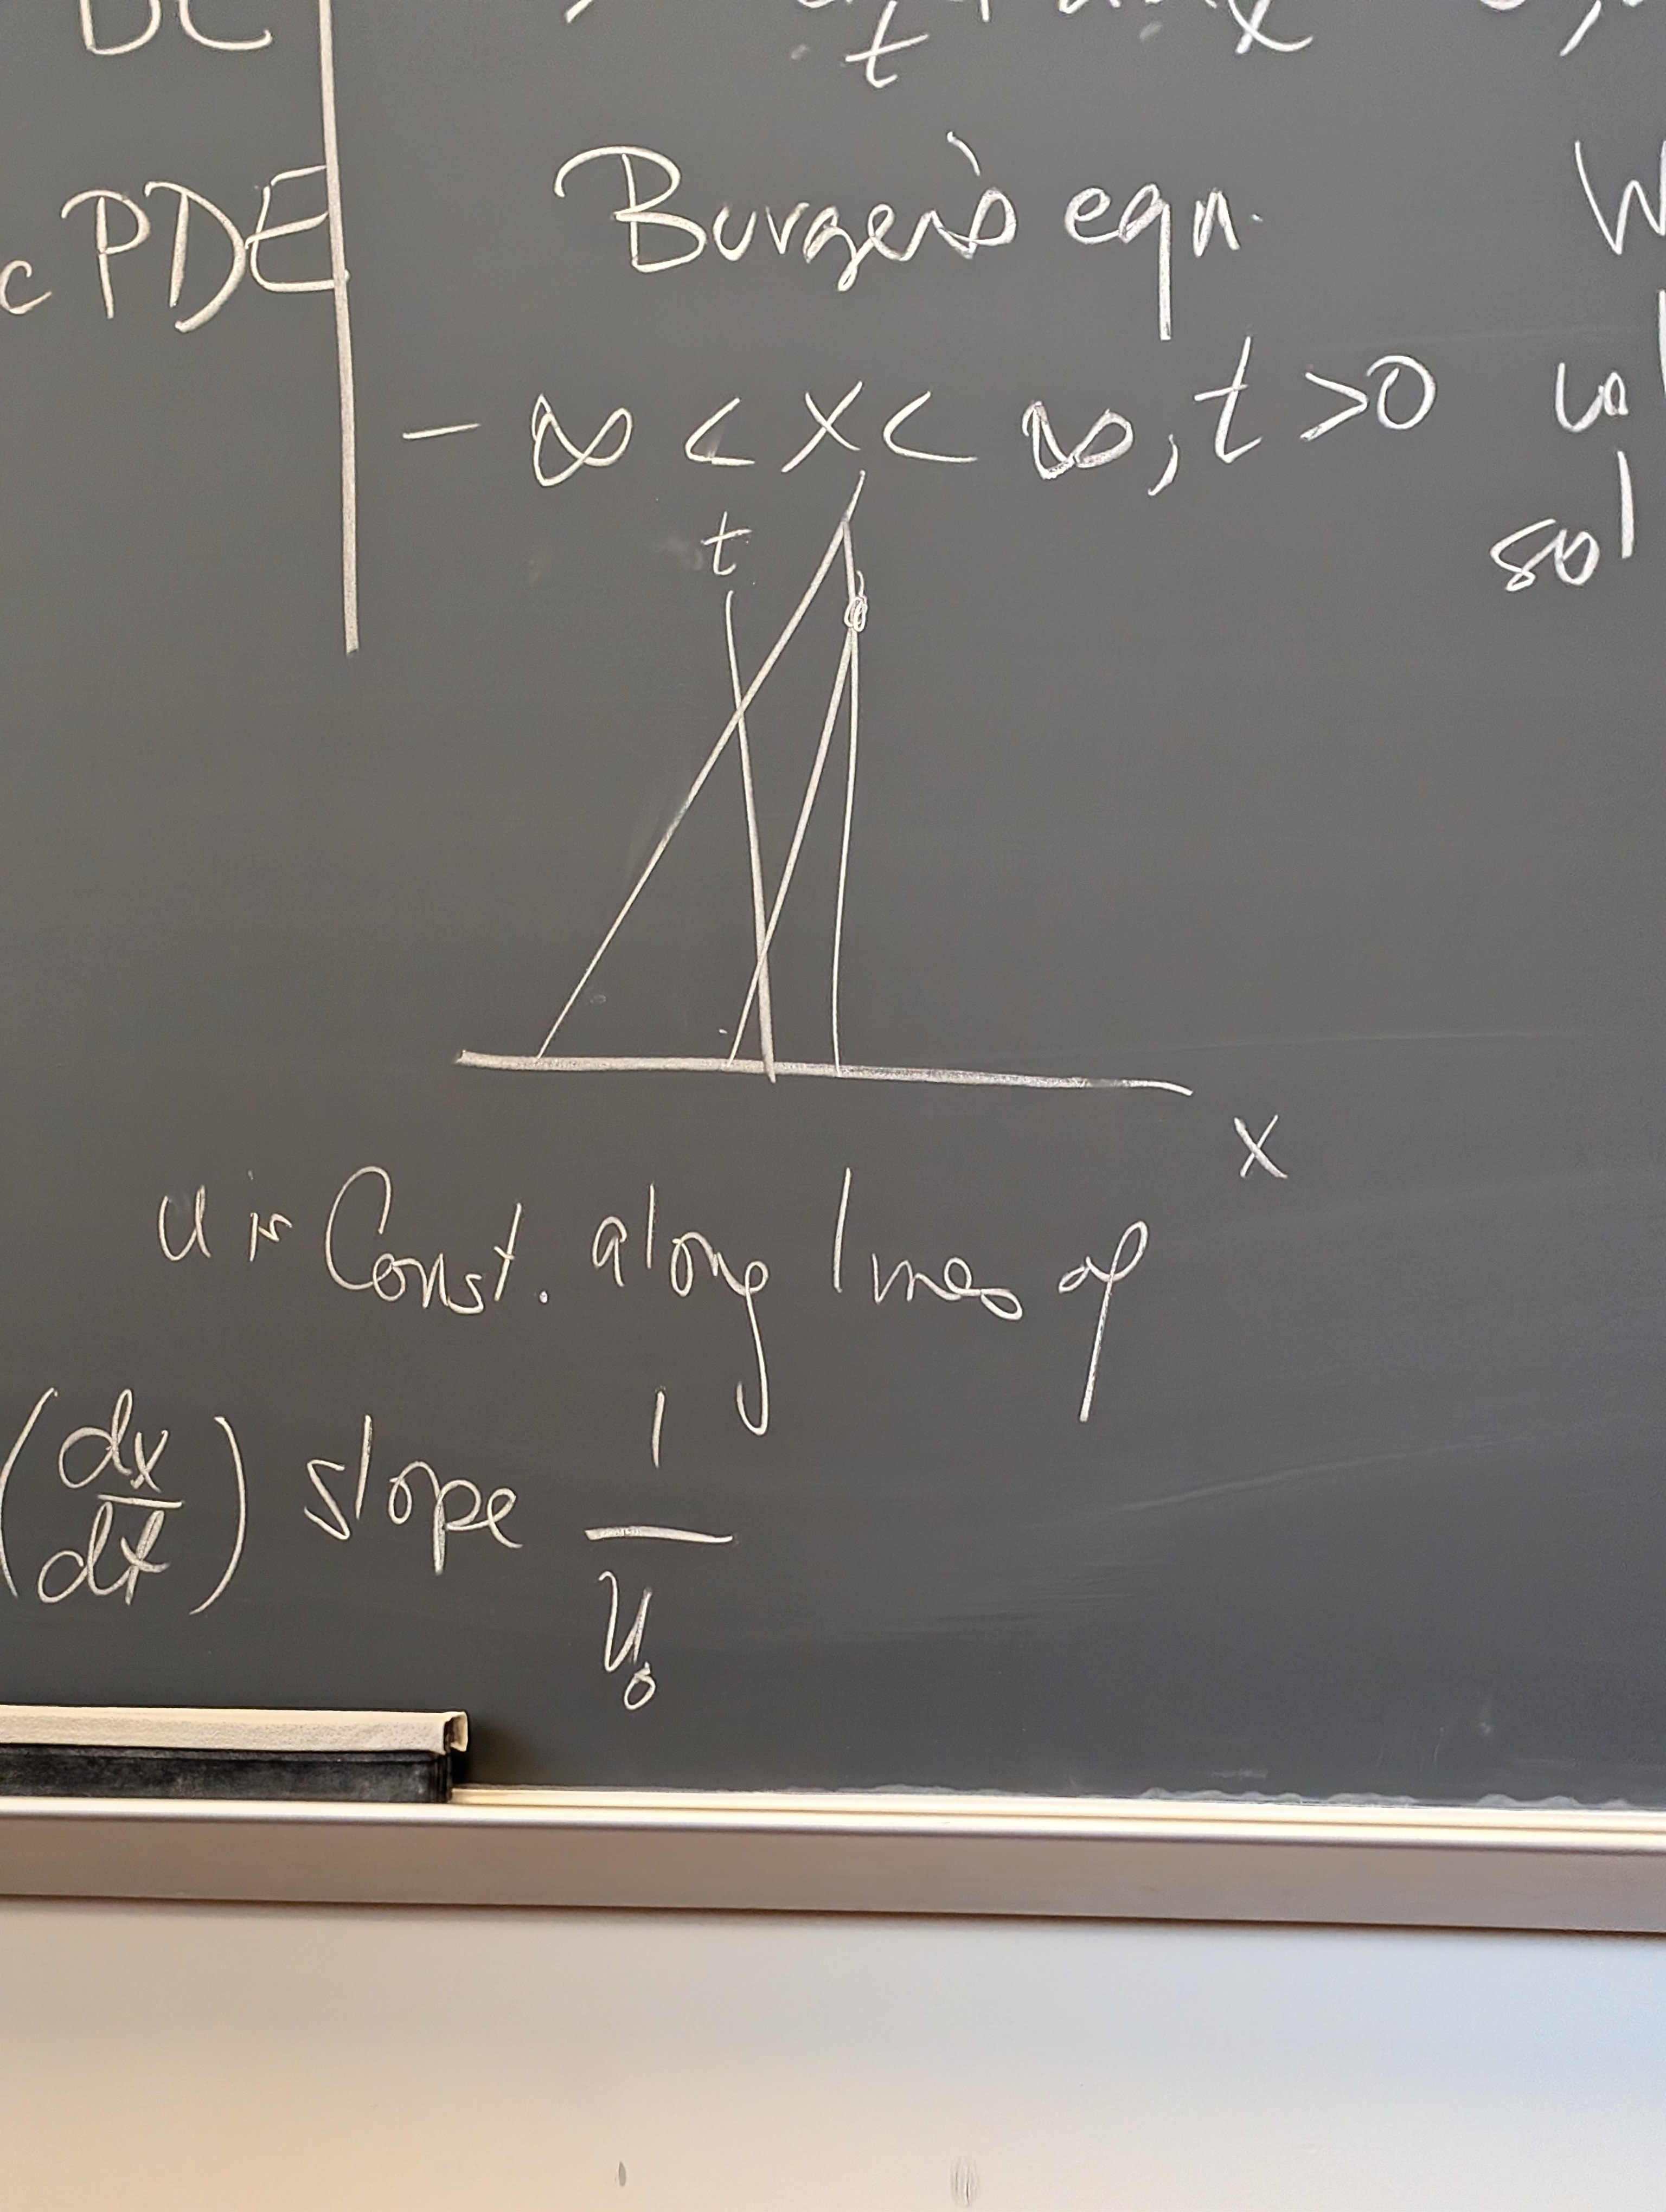
\includegraphics[width=0.5\textwidth]{img/PXL_20240826_154416711}
    \caption{Burger's Equation}
    \label{fig:burger}
\end{figure}    

Can also happen that a classical solution does exists, BUT it is easiest to find a weak solution.

- Find a weak solution

- Show it's classical (regularity theory)

For linear elliptic PDE's ex. Laplace's Equation,

\[
    \Delta u = u_{x_1 x_1} + \dots + u_{x_n x_n} = 0
\]

in \(\Omega \subset \mathbb{R} ^n\) 

A weak solution satisfies the equation obtained through multiplication by a test function \(C^{\infty} _c\) and integrate by parts

ie take any \(\phi\in C^{\infty} _c(\Omega )\) 

\(\int_{\Omega }^{} \phi \Delta u = 0\) 

\(= - \int_{\Omega }^{} \nabla \phi \cdot \nabla u + \int_{\partial \Omega }^{} \phi \nabla u \cdot \nu \) 

Note that the second term is integrated over the boundary. So it goes to \(0\)

So, if:

\[
    \int_{\Omega }^{} \nabla \phi \cdot \nabla u = 0 \forall \phi\in C_c^{\infty}
\]

We say \(u\) weakly solves Laplace's equation because it requires only one derivative (not two).

\begin{definition}
    [Weak Derivative]

    A locally integrable function \(u\) [notationally \(u\in L^1_{loc} (\Omega)\)] has a weak \(x_i\) derivative \(v\) if \(v\) is locally integrable and 

    \(\int_\Omega u \phi_{x_i} \, \mathrm{d} x = - \int_\Omega v \phi \,\mathrm{d} x \) for all \(\phi\in C_c^{\infty} (\Omega)\)  
\end{definition}

\(u\) and \(v\) can be terrible near the boundary but \(\phi\) vanishes so we don't care!

Recall: Multi-inde notation

If \(u:\mathbb{R} ^n \to \mathbb{R} \) and \(\alpha = (\alpha _1, \dots , \alpha _n)\) where \(\alpha _j\) is non-negative integer then,

\[
    D^\alpha u = \frac{\partial ^{\vert \alpha  \vert }}{\partial ^{\alpha _1}_{x_1}\dots \partial ^{\alpha _n}_{x_n}}
\]

eg in \(\mathbb{R} ^3\) for \(\alpha =(1,2,1)\) then \(D^\alpha u = u_{x_1 x_2 x_2 x_3}\) 

\begin{definition}
    Given \(u,v\in L_{loc}^1(\Omega), \Omega \subset \mathbb{R} ^n\) and \(\alpha \) a multi-index, we say \(v\) is the weak \(\alpha \)th derivative of \(u\) if integration by parts works:

    if \(\int_{\Omega }^{} u D^\alpha \phi \,\mathrm{d}x = (-1)^{\vert \alpha  \vert} \int_{\Omega }^{} v \phi \,\mathrm{d}x, \forall \phi \in C_c^{\infty} (\Omega)\) 
\end{definition}

If we are define weak anything, if our weak thing actually happened to be good, we want it to satisfy the strong definition as well! For example if differentiation is allowed, then integration by parts would actually work. So, if \(u\) were smooth, then our derivative would actually satisfy the solution, since

\[
    \int_{\Omega }^{} (D^\alpha u - v) \phi \,\mathrm{d}x = 0
\]

So \(D^\alpha u = v\) almost everywhere. 

Recall: \(u\in L^p(\Omega), p > 0\) if \(\int \vert u \vert ^p \,\mathrm{d} x < \infty\) 

\(u\in L^p_{loc}(\Omega)\) if \(\forall \Omega_1 \subset \subset \Omega, \int _{\Omega _1}\vert u \vert ^p \, \mathrm{d} x < \infty \) 

\subsection*{Sobolev Spaces}

\begin{definition}
    [Sobolev Spaces] Fix \(1 \leq p \leq \infty\) and a non-negative integer \(k\). Let \(\Omega \subset \mathbb{R} ^n\) be open.

    Then the \underline{Sobolev space} \(W^{k,p}(\Omega)\) consists of all functions \(u\in L^1_{loc}(\Omega)\) such that for every multi-index \(\alpha\) with \(\vert \alpha  \vert < k\), \(D^\alpha u\) exists weakly and lies in \(L^p(\Omega)\).
\end{definition}

Example 1: Consider \(\tilde{u}(x) = \vert x \vert \). Doesn't have a derivative. What about weak derivative?

Claim: \(u\) has weak 1st derivative \(v(x) = \begin{dcases}
    -1, &\text{ if } x < 0 ;\\
    1, &\text{ if } x > 0 ;\\
\end{dcases}\) 

We verify that using test function.

Let \(\phi \in C_c^{\infty} (\mathbb{R})\) 

\[
    LHS = \int_{-\infty}^{\infty} v(x)\phi(x) \,\mathrm{d}x = - \int_{-\infty}^{0} \phi(x) \,\mathrm{d}x + \int_{0}^{\infty} \phi(x) \,\mathrm{d}x 
\]

\[
    RHS = - \int_{-\infty}^{\infty} \tilde{u}(x)\phi^{\prime} (x) \,\mathrm{d}x = \int_{-\infty}^{0} x \phi^{\prime} (x) \,\mathrm{d}x - \int_{0}^{\infty} x \phi^{\prime} (x) \,\mathrm{d}x 
\]

By applying IBP

\[
    RHS = - \int_{-\infty}^{0} \phi(x) \,\mathrm{d}x + \int_{0}^{\infty} \phi(x) \,\mathrm{d}x 
\]

[boundary terms don't matter because either \(x\) or \(\phi \) vanishes]

Since \(\vert x \vert\) is locally integrable for any \(p\), \(\tilde{u}\in W_{loc}^{1,p}(\mathbb{R})\) for all \(p\) 

Example 2: Consider the Heaviside function

\[
    u(x) = \begin{dcases}
        1, &\text{ if } x > 0 ;\\
        0, &\text{ if } x < 0 ;
    \end{dcases}
\]

Is NOT going to be weakly differentiable!


\section*{Wednesday, 8/28/2024}

\subsection*{Sobolev Space \(W^{k,p}(\Omega)\) }

\(u \in W^{k,p}(\Omega)\) if


\(D^\alpha u \in L^p\) weakly for all \(\alpha \) such that \(\vert \alpha  \vert \leq k\) 

This is a normed space.

\[
    \lVert u \rVert _{W^{k,p}(\Omega)} = \left[ \sum_{\vert \alpha  \vert \leq k} \int_\Omega \vert D^\alpha u \vert ^p \right] ^{\frac{1}{p}}
\]

If \(p = \infty\) we just take the sup norm.

We have convergence: \(\{ u_j \} \subset W^{k,p}(\Omega)\) converges in \(W^{k,p}\)

to \(u\in W^{k,p}(\Omega)\) if \(\left\vert u_j - u \right\vert _{W^{k,p}(\Omega)} \to 0\) as \(j \to \infty\)  

\begin{definition}
    \(W^{k,p}_0(\Omega) \coloneqq \) closure in \(W^{k,p}(\Omega)\)-norm of \(C_o^{\infty}(\Omega)\) 
\end{definition}

\underline{Remark}: \(W^{k,p}(\Omega)\) and \(W^{k,p}_0(\Omega)\) are Banach spaces [normed, complete [since Lp is complete]]

For \(p = 2\) we don't usually use \(W^{k,2}(\Omega)\). We use \(H^k(\Omega)\). \(H\) is for Hilbert. This is a Hilbert space [there exists an inner product].

\[
    (u,v)_{H^k(\Omega)} \coloneqq \sum_{\vert \alpha  \vert \leq k} \int_{\Omega}^{} D^\alpha u D^\alpha v
\]

H\"older's inequality implies:

\[
    \left\vert \int _\Omega D^\alpha u D^\alpha v \right\vert \leq \lVert D^\alpha u \rVert _{L^2} \lVert D^\alpha v \rVert _{L^2}
\]

Let's go back to the example.

Let \(u(x)\) be the heaviside function, \(0\) for negative, \(1\) for positive. Is it weakly differentiable? Is it in some sobolev space?

Is \(u\in W^{k,p}(\mathbb{R})\) for some \(k\) and \(p\)? Does \(u\) have a weak solution?

Answer: \underline{No}! We use contradiction.

Suppose there is such a \(v\in L^1_{loc}(\mathbb{R})\) such that IBP holds:

\[
    \int_\mathbb{R} u \phi^{\prime} \, \mathrm{d} x = - \int _\mathbb{R} v \phi \, \mathrm{d} x
\]

for all \(\phi\in C_c^{\infty} (\mathbb{R})\) 

Then, \(\int_{0}^{\infty} \phi^{\prime} (x) \,\mathrm{d}x = - \int_{-\infty}^{\infty} v \phi \,\mathrm{d}x \) 

Therefore, \(\phi(0) = \int_{-\infty}^{\infty} v(x)\phi(x) \,\mathrm{d}x \) 

We use this for contradiction. Consider a sequence \(\{ \phi_j \} \) of test functions so that \(\phi_j(0)=1\) for all \(j\) and \(0 \leq \phi_j(x) \leq 1\) for all \(x\).

Further suppose that the support for \(\phi_j\) shrinks to the origin. 

\[
    \phi_j(0) = 1 = -\int_\mathbb{R} v\phi_j \, \mathrm{d} x
\]

Now, \(v\phi_j \to 0\) pointwise a.e.

\(\vert v \phi_j \vert \leq \vert v \vert \in L^1_{loc}\) 

This gives us the desired contradiction.

\underline{Notice}: \(\phi(0)=\int v(x)\phi(x)\) is true for the `function' dirac delta. This is not really a function, this is a distribution.

Moral of the story: We can't have too big of a discontinuity [here we have a jump discontinuity] and still be in Sobolev spaces.

Example: \(f(x) = \frac{1}{\vert x \vert ^\alpha}\) for \(x\in B(0,1) = \{ x\in\mathbb{R} ^n : \vert x \vert < 1 \} \) and \(\alpha > 0\)

For which \(k,p,n,\alpha\) is \(f\in W^{k,p}(B(0,1))\)? 

Question 1: Is this in any Lp space? If no then game over.

Is \(f\in L^p(B(0,1))\) 

\[
    \int_{B(0,1)}^{} \frac{1}{\vert x \vert ^{\alpha p}} \,\mathrm{d}x = \int_{0}^{1} \int_{\partial B(0,r)}^{} \frac{1}{\vert x \vert ^{\alpha p}} \,\mathrm{d}S  \,\mathrm{d}r 
\]

\[
    = \int_{0}^{1} \frac{1}{r^{\alpha p}} \mu (\partial B(0,r)) \,\mathrm{d}r 
\]

\[
    = \omega_n \int_{0}^{1} \frac{1}{r^{\alpha p}}r^{n-1} \,\mathrm{d}r = \omega _n \int_{0}^{1} r^{-\alpha p + n - 1} \,\mathrm{d}r 
\]

So, \(f\in L^p\) if \(\alpha p \leq n\) 

Note that \(\vert D^\alpha f \vert \leq L^p\) for \(\vert \alpha  \vert = 1\) provided \((\alpha +1)p \leq n\) 

Is \(f\) weakly differentiable for \(\vert \alpha  \vert = 1\)?

Consider \(\epsilon < 1\) 

\[
    \int_{B(0,1) \setminus B(0,\epsilon)}^{} f \phi_{x_i} \,\mathrm{d}x = \int_{B(0,1)\setminus B(0,\epsilon)}^{} \nabla \cdot (0, 0, f\phi, 0, 0) \,\mathrm{d}x - \int_{B(0,1) \setminus B(0,\epsilon)}^{} \phi f_{x_i} \,\mathrm{d}x 
\]

\[
    \int_{B(0,1)\setminus B(0,\epsilon)}^{} f \phi_{x_i} \,\mathrm{d}x = - \int_{B(0,1)\setminus B(0,\epsilon)}^{} \phi f_{x_i} \,\mathrm{d}x + \int_{\partial (B(0,1)\setminus B(0,\epsilon ))} f \phi \nu_i \,\mathrm{d}S 
\]

Note that the outer normal dissapears, we only have the inner normal.

\[
    \int_{\partial (B(0,1)\setminus B(0,\epsilon ))}^{} f \phi \nu _i \,\mathrm{d}S = \int_{\partial B(0,\epsilon)}^{} f \phi \nu_i \,\mathrm{d}S
\]

Setting \(\epsilon \to 0\) we see that the integral converges. Also,

\[
    \left\vert \int_{\partial (B(0,1)\setminus B(0,\epsilon))}^{} f \phi \nu_i \,\mathrm{d}S  \right\vert \leq \int_{\partial B(0,\epsilon)}^{} \vert f \phi \nu_i \vert \leq c \int_{\partial B(0,\epsilon)}^{} \vert f \vert  \,\mathrm{d}S \leq \frac{c}{\epsilon^\alpha} \omega_n \epsilon^{n-1} \to 0
\]

provided \(n - 1 \geq \alpha\) 

So,

\[
    \int_{B(0,1)}^{} f \phi_{x_i} \,\mathrm{d}x = - \int_{B(0,1)}^{} \phi f_{x_i} \,\mathrm{d}x 
\]

So \(f\) is weakly differentiable for \(\vert \alpha  \vert = 1\) 

(See Appendix 5 in Evans)

Mollification:

There are lot of situation in PDE where you have a function and you don't know how nice is it in terms of derivative. So you convolve it so that it is nice and take some limit.

Let \(\eta\) satisfy \(\eta \in C_c^{\infty} (\mathbb{R}^n)\)

Suppose \(\eta \equiv 0\) for \(\vert x \vert \geq 1\) 

\(\int_{\mathbb{R} ^n}^{} \eta (x) \,\mathrm{d}x = 1\) 

Suppose \(\eta \) is radial, \(\eta = \eta (\vert x \vert)\) just a function of radial distance

Note that there is no such analytic function. But there are infinitely differentiable ones.

Define \(\eta_{\epsilon} \coloneqq \epsilon^{- n} \epsilon(\frac{x}{\epsilon})\) 

So we rescale the function.

Then given \(u \in L^1_{loc}(?)\) we define the mollification

\[
    u_{\epsilon}(x) = u \ast \eta _\epsilon = \int_{}^{} u(x-y) \eta_{\epsilon } (y) \,\mathrm{d}y = \int_{}^{} u(y) \eta _\epsilon (x-y) \,\mathrm{d}y 
\]


\section*{Friday, 8/30/2024}

Given \(\Omega \subset \mathbb{R} ^n\), open, bounded

\(\forall \epsilon\) define \(\{ x\in \Omega : \text{dist} (x, \partial \Omega ) > \epsilon \} = \Omega_{\epsilon} \) 

Let \(\eta \in C_c^{\infty} (\mathbb{R}^n)\) such that

\(0 \leq \epsilon \leq 1\) and \(\int_{B(0,1)}^{} \eta (x) \,\mathrm{d}x = 1\) and \(\mathop{\mathrm{supp}}(\eta) \subset \overline{B(0,1)} \) 

Define \(\eta_{\epsilon}(x) \coloneqq \epsilon ^{-n} \eta(\frac{x}{\epsilon}) \) 

Then, \(\mathop{\mathrm{supp}}(\eta _\epsilon) \subset \overline{B(0,\epsilon)} \) 

\[
    \int_{B(0,\epsilon)}^{} \eta _\epsilon (x) \,\mathrm{d}x = \epsilon ^{-n} \int_{B(0,\epsilon)}^{} \eta (\frac{x}{\epsilon }) \,\mathrm{d}x = \int_{B(0,1)}^{} \eta (x) \,\mathrm{d}x = 1
\]

\begin{theorem}
    Given \(f\in L^1_{loc}(\Omega)\) define \(f_{\epsilon} \coloneqq \eta_{\epsilon} \ast f \) for \(x\in \Omega_{\epsilon} \) 
    
    \[
       f_{\epsilon}(x)  = \int_\Omega \eta_{\epsilon} (x-y) f(y) \, \mathrm{d} y
    \]

    Then, i: \(f_{\epsilon}(x)\) is infinitely differentiable.

    ii: \(f_{\epsilon} \to f \) pointwise a.e.
    
    iii: If \(f\) is continuous then \(f_{\epsilon} \to f\) uniformly on compact subsets of \(\Omega\) 

    iv: If for \(1 \leq p < \infty, f\in L^p(\Omega)\) then \(f_{\epsilon} \to f\) in \(L^p(\Omega)\). Also true for \(f\in L_{loc}^p\) 
\end{theorem}

\begin{proof}
    (i): Convolution is a child, and it inherits the nicest properties of the parent. \(\eta_{\epsilon}\) is nicer.

    Idea: it is legal to bring derivatives inside the integral. 

    \[
        \frac{f_{\epsilon}(x + he_i) - f_{\epsilon}(x)}{h} = \int_{\Omega }^{} \left[ \frac{\eta_{\epsilon} (x+he_i - y) - \eta_{\epsilon} (x-y)}{h} \right] f(y) \,\mathrm{d}y 
    \]

    Stuff in brackets converges uniformly in \(y\) to \(\eta_{\epsilon _{x_i}} (x-y)\) using Taylor remainder theorem.

    Then Lebesgue Dominated Convergence finishes the job.

    (iii) Fix \(K \subset \Omega\) where \(K\) compact.

    \(\forall x\in K\) we have \(\vert f_{\epsilon } (x) - f(x) \vert = \left\vert \int_{\Omega} (\eta_{\epsilon} (y) f(x-y)) \,\mathrm{d}y - f(x) \right\vert  \) 

    \[
        = \left\vert \int_{\Omega} \eta_{\epsilon} (y) \left[ f(x-y) - f(x) \right]  \,\mathrm{d}y  \right\vert 
    \]

    \[
        \leq \int_{\Omega} \eta_{\epsilon } (y) \left\vert f(x-y) - f(x) \right\vert  \,\mathrm{d}y 
    \]

    Since \(K\) is compact, \(f\) is uniformly continuous on \(K\).

    So, \(\forall \beta > 0\) we have \(\epsilon_0\) such that \(\forall \epsilon < \epsilon _0\) such that \(\forall x,y\) such that \(\vert y \vert < \epsilon\) we have \(\vert f(x-y) - f(x) \vert < \beta\) 

    So,

    \[
        \leq \int_{\Omega} \eta_{\epsilon}(y) \beta  \,\mathrm{d}x = \beta 
    \]

\end{proof}

What is the relevance to Sobolev spaces?

Often we are going to try to prove some estimates. We want to prove some inequalities.

Then, we mollify and prove it for the mollification. If we mollify a Sobolev function, we get an approximation.

\begin{theorem}
    [Local Approximation Away from \(\partial \Omega\)]

    Assume \(u \in W^{k,p}(\Omega)\) [aka function has \(k\)'th weak derivatives which are locally integrable in order \(p\)]. Define \(u_{\epsilon} = \eta_{\epsilon } \ast u \) in \(\Omega_{\epsilon } = \{ x\in \Omega : \text{dist} (x,\partial \Omega ) > \epsilon \} \) 
    
    THen, \(u_{\epsilon} \in C^{\infty}(\Omega_{\epsilon} )\) 

    And \(u_{\epsilon } \to u\) in \(W_{loc}^{k,p}(\Omega)\) 
\end{theorem}

\begin{proof}

    Note infinite derivative we already have by property of mollification.

    Fix the multi-index \(\alpha\) suh that \(\vert \alpha \vert \leq k\).

    \underline{Claim 1}: \(D^\alpha u_{\epsilon} = \eta_{\epsilon} \ast D^\alpha u \)
    
    In other words, mollification and derivatives commute.

    To see this, consider \(x\in \Omega_{\epsilon} \)

    \[
        D^\alpha u_{\epsilon} = D^\alpha \int_{\Omega} \eta _\epsilon (x-y) u(y) \,\mathrm{d}y 
    \]

    \[
        = \int_{\Omega} D^\alpha_x \eta_{\epsilon} (x-y) u(y) \,\mathrm{d}y 
    \]

    \[
        = (-1)^{\vert \alpha  \vert } \int_{\Omega} D^\alpha_y \eta_{\epsilon} (x-y) u(y) \,\mathrm{d}y 
    \]

    \[
        = (-1)^{\vert \alpha \vert } (-1)^{\vert \alpha \vert } \int_{\Omega} \eta_{\epsilon} (x-y) D^\alpha u(y) \,\mathrm{d}y 
    \]

    \[
        = \eta_{\epsilon } \ast D^\alpha u
    \]

    proving the claim.

    Now, fix \(V \subset \Omega\) with open \(\overline{V} \subset \Omega\) (\(V \subset \subset \Omega\) )

    Apply previous theorem, item iv and the claim

    \(D^\alpha u_{\epsilon} \to D^\alpha u\) in \(L^p(V)\) for all \(\alpha \) such that \(\vert \alpha  \vert \leq k\) 

\end{proof}

\begin{theorem}
    [Global Approximation]

    Theme:

    Sobolev can be approximated by smooth sobolev

    Let \(\Omega \subset \mathbb{R}^n\) be open, bounded. Assume \(u\in W^{k,p}(\Omega)\) for \(1 \leq p < \infty\) 
    
    Then, \(\exists \{ u_m \} \subset C^{\infty}(\Omega) \cap W^{k,p} (\Omega)\) [infinitely smooth AND sobolev] such that \(u_m \to u\) in \(W^{k,p}(\Omega)\). Meaning:

    \[
        \lim_{m \to \infty} \left\lVert u_m - u \right\rVert _{W^{k,p}(\Omega)} \to 0
    \]

\end{theorem}

Idea of Proof: 

\begin{figure}[H]
    \centering
    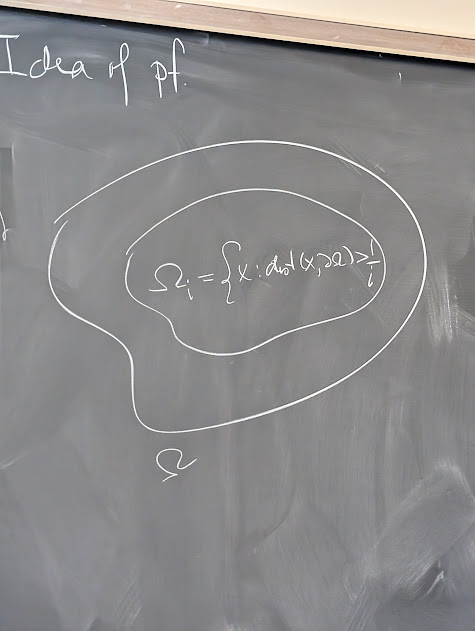
\includegraphics[width=0.4\textwidth]{img/PXL_20240830_161621740}
\end{figure}

We have a bunch of \(\Omega _i\) with \(\bigcup_{i=1}^{\infty} \Omega _i = \Omega\) 

Use a partition of unity \(\{ \phi_i \} \) so that \(\sum_{} \phi_i(x) = 1\), mollify.

Proof is on Evans.

\section*{Wednesday, 9/4/2024}

\subsection*{Traces}

We are going to solve PDEs using Sobolev spaces. We typically specify boundary conditions in PDEs. But in first glance, since Sobolev functions are defined upto a set of measure zero, it seems ill suited to dealing with boundary conditions [since boundary \(\partial \Omega\) has measure 0].

How to define boundary values for a Sobolev functions?

We are going to establish an inequality for smooth function.

\begin{theorem}
    Assume \(\partial \Omega\) is \(C^1\) surface\footnote{meaning \(\partial \Omega\) can be described as the graph of a \(C^1\) function.}. Then \(\exists\) a bounded linear operator \(T : W^{1,p}(\Omega) \to L^p(\partial \Omega)\) for \(1 \leq p < \infty\) such that:

    \begin{enumerate}[label=\roman*)]
        \item \(Tu = u |_{\partial \Omega}\) if \(u \in W^{1,p}(\Omega)\cap C(\overline{\Omega})\) 
        \item \(\left\lVert T u \right\rVert _{L^p(\partial \Omega)} \leq C \left\lVert u \right\rVert _{W^{1,p}(\Omega)}\) for some \(C= C(p, \Omega)\)   
    \end{enumerate} 
\end{theorem}

\begin{proof}

    Outline:

    \begin{enumerate}[label=\arabic*)]
        \item Fix \(x_0 \in \partial \Omega\). Suppose \(\partial \Omega\) is `flat' near \(x_0\). In fact, define ball \(B\) centered at \(x_0\) such that inside \(B\), \(\partial \Omega\) is flat.
        
        [insert picture]

        Then we can define \(x^{\prime}  = (x_1, \cdots , x_{n-1})\). If the last coordinate is positive, we are inside \(\Omega\).

        Inside \(B\), \(\partial \Omega\) is flat. we can define \(B^{\prime} \subset B\) centered at \(x_0\).

        Let \(\zeta \in C_0^{\infty} (B)\) so that \(\zeta \equiv 1\) on \(B^{\prime}\) and \(\zeta \geq 0\).

        Define \(\Gamma \coloneqq \partial \Omega \cap B^{\prime}\).
        
        Assume \(u \in C^1(\overline{\Omega })\).

        \[
            \int_{\Gamma}^{} \vert u \vert ^ p \,\mathrm{d}x ^{\prime} \leq \int_{\{ x_n = 0 \} \cap B}^{} \zeta\vert u \vert ^p \,\mathrm{d}x^{\prime}  
        \]

        \[
            = - \int_{\{ x_n = 0 \} \cap B}^{} (0, \cdots , 0, \zeta \vert u \vert ^ p) \cdot (0, \cdots , 0, -1) \,\mathrm{d}x^{\prime} 
        \]

        We are almost set up for divergence theorem. Since \(\zeta = 0\) on the boundary of \(B\), we actually have the whole boundary! Applying the divergence theorem, we get:

        \[
            = - \int_{B \cap \Omega}^{} \frac{\partial}{\partial x_n} \left[ \zeta (x) \vert u(x) \vert ^ p \right]  \,\mathrm{d}x 
        \]

        \[
            = - \int_{B \cap \Omega}^{} \left[ \zeta_{x_n} \vert u \vert ^ p + \zeta p \vert u \vert ^{p-1} \frac{u}{\vert u \vert } u_{x_n} \right] \,\mathrm{d}x 
        \]

        \[
            = - \int_{B \cap \Omega}^{} \left[ \zeta_{x_n} \vert u \vert ^ p + \zeta p \vert u \vert ^{p-1} \sgn(u) u_{x_n} \right] \,\mathrm{d}x 
        \]

        Now we use \underline{Young's Inequality}.
        
        \begin{theorem}
            [Young's Inequality]

            For any \(a, b > 0\) and \(p, q\) such that \(\frac{1}{p} + \frac{1}{q} = 1\), we have:

            \[
                ab \leq \frac{a^p}{p} + \frac{b^q}{q}
            \]
        \end{theorem}

        We are estimating abolute value, so we can take absolute value. Using Young's inequality on \(a = \vert u_{x_n} \vert\) and \(b = \vert u \vert ^{p-1}\),

        \[
            \int_{\Gamma}^{} \vert u \vert ^ p \,\mathrm{d}x^{\prime} 
        \]

        \[
            \leq \int_{B }^{\infty} \left[ \vert \zeta_{x_n} \vert \vert u \vert ^ p + p \vert \zeta  \vert \left[ \frac{(\vert u \vert ^{p-1})^{p / (p-1)}}{p / (p-1)} + \frac{\vert u_{x_n} \vert ^{p}}{p} \right]  \right]  \,\mathrm{d}x 
        \]

        \[
            \leq C \int_{B \cap \Omega}^{} \left[ \vert u \vert ^ p + \vert \nabla u \vert ^ p \right] \,\mathrm{d}x \leq C \int_{\Omega}^{} \left[ \vert u \vert ^ p + \vert \nabla u \vert ^ p \right]  \,\mathrm{d}x 
        \]

        Now, \(\partial \Omega \in C^1\) means, centered at any point \(x_0 \in \partial \Omega\) \(\partial \Omega\) can be written as a graph \(x_n = f(x^{\prime})\) where \(\vert f \vert_{C_1}\) is bounded.\footnote{\(\vert f \vert_{C_1}= \sup \vert f \vert + \sup \vert \nabla f \vert \)}

        Therefore, Ball inside of which \(\partial \Omega\) is a graph has radius \(R\) depending on \(C^1\) norm.

        \item For the next step, we flatten the boundary of \(\Omega\) by a change of variables.
        
        [insert picture]

        [insert picture 2]

        Change variables: \(y = (y^{\prime} , y_n)\).

        Set \(y^{\prime}  = x^{\prime} \) 

        \(y_n \coloneqq x_n - f(x^{\prime})\) 

        \(y = G(x)\).

        So, \(y_n = 0\) means \(x_n = f(x^{\prime})\), which means \underline{we're on the graph}.

        We can think of this in terms of the \underline{Inverse Function Theorem}. What is the Jacobian of \(G\)?

        \[
            \operatorname{Jac}(G) = \det \nabla G = \det \begin{pmatrix}
                I &  &  0 \\
                 &  &  \vdots \\
                -f_{x_1} - f_{x_2} - \cdots - f_{x_{n-1}} &  &  1 \\
            \end{pmatrix} = 1
        \]

        So, \(G ^{-1}\) is \(C^1\).

        Then, \(\vert \nabla G \vert \leq C (\partial \Omega)\) and \(\vert \nabla(G ^{-1} ) \leq C(\partial \Omega) \vert \).

        \(u\) is a given function. We can define a new function that has a flat boundary which we can use instead of \(u\).

        Define \(\tilde{u}(y) \coloneqq u(G ^{-1} (y))\).

        Then, \(u(x) = \tilde{u}(G(x))\) 

        Suppose \(G(\Gamma) = \tilde{G}\).

        Then, Step 1 implies,

        \[
            \int_{\tilde{\Gamma}}^{} \vert \tilde{u}^p \vert  \,\mathrm{d}y^{\prime}  \leq C \int_{\text{shaded region}}^{} \left[ \vert \tilde{u} \vert ^ p + \vert \nabla \tilde{u} \vert ^ p \right]  \,\mathrm{d}y
        \]

        Where the shaded region is \(\{ x \mid x_n > f(x^{\prime}), x\in B_R \} \). Now,

        \[
            \left\vert \nabla \tilde{u}(y) \right\vert \leq \left\vert D u \cdot \nabla(G ^{-1}) \right\vert \leq C \left\vert \nabla u \right\vert 
        \]

        Continuing,

        \[
            \int_{\tilde{\Gamma}}^{} \vert \tilde{u}^p \vert  \,\mathrm{d}y^{\prime}  \leq C \int_{\text{shaded region}}^{} \left[ \vert \tilde{u} \vert ^ p + \vert \nabla \tilde{u} \vert ^ p \right]  \,\mathrm{d}y
        \]

        \[
            \implies \int_{\Gamma }^{} \vert u \vert ^ p \,\mathrm{d}x^{\prime} \leq C \int_{\Omega \cap B_R}^{} \left[ \vert u \vert ^ p + \vert \nabla u \vert ^ p \right]  \,\mathrm{d}x \leq C \int_{\Omega}^{} \left[ \vert u \vert ^ p + \vert \nabla u \vert ^ p \right]  \,\mathrm{d}x  
        \]

        Which finishes Step 2.

        \item Decompose \(\partial \Omega\) into \(N_R\) pieces, and add them up using Step 2.
        
        Since \(\partial \Omega\) is compact, \(N_R < N(\partial \Omega)\).
        
        [insert picture]

        We have: \(\forall u\in C^1(\overline{\Omega})\),

        \[
            \int_{\partial \Omega}^{} \vert u \vert ^ p \,\mathrm{d}S \leq C(p,\Omega) \int_{\Omega}^{} \left[ \vert u \vert ^ p + \vert \nabla u \vert ^ p \right]  \,\mathrm{d}x 
        \]

    \end{enumerate} 

    Now, suppose \(u \in W^{1,p}(\Omega)\). Approximate \(u\) in \(W^{1,p}\) norm by \(\{ u_m \} \subset W^{1,p}(\Omega) \cap C^1(\overline{\Omega} )\). Then,

    \[
        \underbrace{\left\lVert u_m - u_l \right\rVert _{L^p(\partial \Omega)}}_{\text{cauchy sequence} } \leq C \left\lVert u_m - u_L \right\rVert ^ p _{W^{1,p}}
    \]

    \(RHS \to 0\), so \(LHS \to 0\) for \(m, l \gg 1\).

    Therefoe, \(\exists T u \in L^p(\partial \Omega)\) which is the limit of this cauchy sequence.

\end{proof}

\section*{Friday, 9/6/2024}

A few comments about traces.

Last time: If \(u \in W^{1,p}(\Omega)\) for \(1 \leq p < \infty\) and \(\partial \Omega \in C^1\) , we can define the trace of \(u\) on \(\partial \Omega\), \(Tu \in L^p(\partial \Omega)\) and \(\exists C = C(p, \Omega)\) such that,

\[
    \left\lVert T u \right\rVert _{L^p(\partial \Omega)} \leq C \left\lVert u \right\rVert _{W^{1,p}(\Omega)}
\]

Recall: \(W^{k,p}_0(\Omega) =\) closure of \(C_c^{\infty}(\Omega)\) in the \(W^{k,p}\) norm.

Suppose \(k = 1, u \in W^{1,p}_0(\Omega)\). Then, \(Tu = 0\) on \(\partial \Omega\) 

Also, if \(k > 1\) and \(u \in w_0^{k,p}(\Omega)\), we have \(T u = 0\). 

In fact, \(T(D^\alpha u) = 0 \forall \alpha\) such that \(\vert \alpha  \vert \leq k - 1\). 

\subsection*{Calculus of Variations}

Our objects of interest are \underline{functionals}.

Consider an \underline{integral functional} of the form:

\[
    E(u) = \int_{\Omega }^{} L(x, u, \nabla u) \,\mathrm{d}x
\]

We use \(E\) because this often denotes \underline{Energy}. It comes from physics often.

In that case, we call \(L\) an energy density. It is also often called the \underline{energy density}. 

A fundamental problem is:

Determine the \underline{infimum} of \(E\) among all functions \(u\) in an \underline{admissible} set \(\mathscr{A}\).

We define:

\[
    m \coloneqq \inf_{u\in \mathscr{A}} E(u)
\]

\underline{``First Variation of \(E\)''}

This is the `calculus of variations' version of a derivative.

If \(\Omega \subset \mathbb{R} ^n\) and \(u:\Omega \to \mathbb{R}\),

\[
    L = L(x,z,p)
\]

where: \(x\) is a point in \(\Omega \subset\mathbb{R}^n\) 

\(z\in\mathbb{R} \) [we put \(u\) here]

\(p\in\mathbb{R}^n\) [we put \(\nabla u\) here]

We put \(u\) in \(E\), but we purtrube it a little bit.

Suppose \(u \in \mathscr{A} \), and \(v\) such that \(u + tv \in \mathscr{A}\) for \(\vert t \vert \) small. 

\(E(u + tv)\)

Then, \(t \mapsto E(u+tv)\) is a function \(\mathbb{R} \to \mathbb{R}\). We take derivative and set \(t = 0\) 

\[
    \frac{\mathrm{d}}{\mathrm{d}t} \bigg\vert_{t=0} E(u + tv) = \delta E(u;v)
\]

Note: if \(u\) is a minimum of \(E\), i.e. \(E(u) = m\), then the first variation \(\delta E(u;v) = 0\) for all \(v\) such that \(u + tv \in \mathscr{A}\). 

\begin{definition}
    \(u\) is called a \underline{critical point} of \(E\) in \(\mathscr{A}\) if \(\delta E(u;v) = 0 \forall v\) such that \(u + tv \in \mathscr{A}\). 
\end{definition}

Question: What is true about a critical point \(u\) of an integral functional of form (\(\ast\))?

\[
    0 = \frac{\mathrm{d}}{\mathrm{d}t} \bigg\vert_{t=0} E(u+tv)
\]

\[
    = \frac{\mathrm{d}}{\mathrm{d}t} \bigg\vert_{t=0} \int_{\Omega }^{} L(x, u+tv, \nabla u + t\nabla v) \,\mathrm{d}x 
\]

\[
    = \int_{\Omega}^{} \left[ \frac{\partial L}{\partial z} (x, u, \nabla u) v + \sum_{j=1}^{n} \frac{\partial L}{\partial p_j} (x, u, \nabla u) v_{x_j} \right]  \,\mathrm{d}x 
\]

\[
    = \int_{\Omega}^{} \left[ \frac{\partial L}{\partial z} (x, u, \nabla u) v + \nabla_p L \cdot \nabla_x v \right]  \,\mathrm{d}x 
\]

Applying IBP,

\[
    = \int_{\Omega}^{} \left[ \frac{\partial L}{\partial z} (x, u, Du) - \sum_{j=1}^n \frac{\partial}{\partial x_j} \left( \frac{\partial }{\partial p_j} L(x,u, \nabla u) \right)  \right] v \,\mathrm{d}x 
\]

\[
    + \int_{\partial \Omega}^{} v \nabla_p L(x,u, \nabla u)\cdot \nu \,\mathrm{d}S 
\]

Now, suppose all allowable \(v\)'s are included in \(C_c^{\infty}(\Omega)\) functions. That would make the boundary term \(0\). Then, since we can choose \(v\) however we want, the big integral is \(0\). 

\[
    \sum_{j=1}^{n} \frac{\partial }{\partial x_j} \left[ \frac{\partial}{\partial p_j} L(x, u, \nabla u) \right] = \frac{\partial L}{\partial z} (x,u,\nabla u)
\]

This is a 2nd order PDE. This is called the Euler-Lagrange equation for \(E\).

\underline{Example}: Take \(\displaystyle E(u) = \int_{\Omega }^{} \frac{1}{2} \left\vert \nabla u \right\vert ^2 + W(x,u) \,\mathrm{d}x \)

Here \(L(x,z,p) = \frac{1}{2} \vert p \vert ^2 + W(x,z)\) 

Then, we find the Euler-Lagrangian.

\[
    \frac{\partial L}{\partial p_j} (x,z,p) = \frac{\partial}{\partial p_j} \left[ \frac{1}{2}\vert p \vert ^2 + W(x,u) \right] = p_j
\]

\[
    \frac{\partial L}{\partial p_j} (x, u, \nabla u) = u_{x_j}
\]

Also,

\[
    \frac{\partial L}{\partial z} (x,z,p) = \frac{\partial W}{\partial z} (x,z)
\]

So, the Euler-Lagrangian equation gives us:

\[
    \sum_{j=1}^{n} \frac{\partial}{\partial x_j} (u_{x_j}) = \frac{\partial W}{\partial z} (x,u)
\]

\[
    \Delta u = \frac{\partial W}{\partial z} (x,u)
\]

This is a \underline{Nonlinear Poisson Equation}.

Question: What should we choose \(\mathscr{A}\) to be to make our life easiest?

We want \underline{integration by parts} to be justified, but we want our topology to be weak enough so that finding minimizers is easy.

In the previous example, we have integral of \(\vert \nabla u \vert ^2\). So, ideally we want it to be \(L^2\).

So, in the example, best choice is \(H^1(\Omega)\).

How does one find a minimzer?

\underline{Direct Method}: Our problem is, we want to find \(u \in \mathscr{A}\) such that:

\[
    m \coloneqq \inf_{u\in \mathscr{A}} E(u)
\]

Idea: We find a sequence \(\{ u_j \}\) [called a \underline{minimizing sequence}]: so that \(\{ u_j \} \subset \mathscr{A}\) and \(E(u_j) \to m\).

\underline{Step 1}: Try to get a convergent subsequence of \(u_{j_k} \to u_\ast \in \mathscr{A}\). [Compactness]

In this step, if we choose \(\mathscr{A}\) to be `too strong', we lose. Ideally we want \(\mathscr{A}\) to be sequentally compact.

\underline{Step 2}: \(E\) might not be continuous in this topology, then we don't have \(E(u_\ast)=m\). So, we want \underline{lower semi-continuity}.

\[
    \liminf_{k \to \infty} E(u_{j_k}) \geq E(u_\ast)
\]

Then we have \(E(u_\ast) \leq m\).

This tells us that \(u_\ast\) is a minimum.


\section*{Monday, 9/9/2024}

\begin{theorem}
    [Extension of Sobolev Functions]

    Assume \(\Omega \subset \mathbb{R} ^n\), open , bounded with \(\partial \Omega \in C^1\). Then, \(\exists C = C(p, \Omega)\) and an extension \(E: W^{1,p}(\Omega) \to W^{1,p}(\mathbb{R}^n)\) such that:

    \begin{enumerate}[label=\roman*)]
        \item \(E u = u\) in \(\Omega\)
        \item \(E u\) has compact support
        \item \(\left\lVert E u \right\rVert _{W^{1,p}(\mathbb{R}^n)} \leq C \left\lVert u \right\rVert _{W^{1,p}(\Omega)}\)  
    \end{enumerate} 

\end{theorem}

Idea is, we can let a function down to zero `gently' and extend that way.

\begin{theorem}
    [Gagliardo - Nirenberg - Sobolev Inequality]

    Assume \(1 \leq p < n\). Then, there exists \(C = C(p, n)\) such that for every \(u\in C_0^1(\mathbb{R}^n)\) [compactly supported continuously differentiable function] one has the following inequality:

    \[
        \left\lVert u \right\rVert _{L^{p ^{\ast} }(\mathbb{R}^n)} \leq C \left\lVert \nabla u \right\rVert _{L^p(\mathbb{R}^n)}
    \]

    Where \(p ^{\ast} = \frac{np}{n-p}\) is the \underline{critical sobolev exponent}.

    Note that \(\frac{np}{n-p} = \frac{np-p^2 + p^2}{n-p} = p + \frac{p^2}{n-p} > p\). 
\end{theorem}

\underline{Question}: Where does \(p^{\ast}\) come from?

Given \(u\in C^1_0(\mathbb{R}^n)\), define:

\[
    u_\lambda (x) \coloneqq u(\lambda x)
\]

for \(\lambda > 0\).

Suppose \(\left\vert u \right\vert _{L^q(\mathbb{R}^n)} \leq C \left\vert \nabla u \right\vert _{L^p(\mathbb{R}^n)}\) 

For which \(q\) could this be true? Consider the norm of the scaled function:

\[
    \left\lVert u_\lambda  \right\rVert _{L^q} = \left[ \int_{\mathbb{R} ^n}^{} \vert u(\lambda x) \vert ^ q \,\mathrm{d}x  \right] ^ {\frac{1}{q}} = \frac{1}{\lambda ^{n / q}} \left[ \int_{\mathbb{R}^n}^{} \vert u(y) \vert ^ q \,\mathrm{d}y  \right] ^{\frac{1}{q}}
\]

\[
    \left\lVert \nabla u_\lambda \right\rVert _{L^p} = \left[ \int_{\mathbb{R} ^n}^{} \vert \nabla_x u(\lambda x) \vert ^ p \,\mathrm{d}x  \right] ^{\frac{1}{p}} = \underbrace{\frac{1}{\lambda ^{\frac{n}{p}}} (\lambda ^ p)^{\frac{1}{p}}}_{=\lambda^{1-\frac{n}{p}}} \left[ \int_{\mathbb{R} ^n}^{} \left\vert \nabla _y u(y) \right\vert ^p \,\mathrm{d}y  \right] ^{\frac{1}{p}}
\]

Applying the same inequality,

\[
    \frac{1}{\lambda^{\frac{n}{q}}} \left[ \int_{\mathbb{R} ^n}^{} \vert u(y) \vert ^q \,\mathrm{d}y  \right]^{\frac{1}{q}} \leq C \lambda^{1 - \frac{n}{p}} \left[ \int_{\mathbb{R} ^n}^{} \vert \nabla u(y) \vert ^p \,\mathrm{d}y  \right] ^{\frac{1}{p}} 
\]

\[
    \left\lVert u \right\rVert _{L^q} \leq C \lambda ^{1 - \frac{n}{p} + \frac{n}{q}} \left\lVert \nabla u \right\rVert _{L^p} \quad \forall \lambda > 0
\]

This means \(1 - \frac{n}{p} + \frac{n}{q}\) must be \(0\).

Therefore, \(q = p^{\ast} \) 

So, if the theorem is true we must have the \(q\).

Now we prove the theorem.

\begin{proof}
    First take \(n = 3\).

    Take \(p = 1\).

    \[
        u(x) = \int_{-\infty}^{x_1} u_{x_1} (y_1, x_2, x_3) \,\mathrm{d}y_1 
    \]

    \[
        u(x) = \int_{-\infty}^{x_2} u_{x_2}(x_1, y_2, x_3) \,\mathrm{d}y_2 
    \]

    \[
        u(x) = \int_{-\infty}^{x_3} u_{x_3}(x_1, x_2, y_3) \,\mathrm{d}y_3 
    \]

    Therefore,

    \[
        \vert u(x) \vert \leq \int_{-\infty}^{x_1} \vert \nabla u(y_1, x_2, x_3) \vert  \,\mathrm{d}y_1 
    \]

    \[
        \vert u(x) \vert \leq \int_{-\infty}^{x_2} \vert \nabla u(x_1, y_2, x_3) \vert  \,\mathrm{d}y_2 
    \]

    \[
        \vert u(x) \vert \leq \int_{-\infty}^{x_3} \vert \nabla u(x_1, x_2, y_3) \vert  \,\mathrm{d}y_3 
    \]

    Multiplying, \(\vert u(x) \vert ^3\) 
    
    \[
        \leq \left[ \int_{-\infty}^{x_1} \vert \nabla u(y_1, x_2, x_3) \vert  \,\mathrm{d}y_1 \right] \left[ \int_{-\infty}^{x_2} \vert \nabla u(x_1, y_2, x_3) \vert  \,\mathrm{d}y_2 \right] \left[ \int_{-\infty}^{x_3} \vert \nabla u(x_1, x_2, y_3) \vert  \,\mathrm{d}y_3 \right] 
    \]

    Therefore, \(\vert u(x) \vert ^{\frac{3}{2}} \leq \) 

    \[
        \underbrace{\left[ \int_{-\infty}^{\infty} \vert \nabla u(y_1, x_2, x_3) \vert  \,\mathrm{d}y_1 \right]^{\frac{1}{2}}}_{=I_1(x_2, x_3)} \underbrace{\left[ \int_{-\infty}^{\infty} \vert \nabla u(x_1, y_2, x_3) \vert  \,\mathrm{d}y_2 \right]^{\frac{1}{2}}}_{=I_2(x_1,x_3)} \underbrace{\left[ \int_{-\infty}^{\infty} \vert \nabla u(x_1, x_2, y_3) \vert  \,\mathrm{d}y_3 \right]^{\frac{1}{2}}}_{=I_3(x_1,x_2)}
    \]

    Integrating with respect to \(x_1\) and applying H\"older,

    \[
        \int_{-\infty}^{\infty} \vert u(x) \vert ^{\frac{3}{2}} \,\mathrm{d}x_1 \leq (I_1(x_2, x_3))^{\frac{1}{2}} \left[ \int_{-\infty}^{\infty} I_2(x_1, x_3) \,\mathrm{d}x_1  \right] ^{\frac{1}{2}} \left[ \int_{-\infty}^{\infty} I_3(x_1, x_2) \,\mathrm{d}x_1  \right] ^{\frac{1}{2}}
    \]

    repeat for \(x_2\) and \(x_3\) and use the fact:

    \[
        \int \vert f \vert \vert g \vert \leq \left[ \int f^2 \right] ^{\frac{1}{2}} \left[ \int g^2 \right] ^{\frac{1}{2}  }
    \]

    We see that,

    \[
        \iiint _{\mathbb{R} ^3} \vert u(x) \vert ^\frac{3}{2} \, \mathrm{d} x \leq \left[ \iiint _{\mathbb{R} ^3} \vert \nabla u(x) \vert \,\mathrm{d} x \right] ^{\frac{3}{2}}
    \]

    Therefore, \(\left\lVert u \right\rVert _{L^{\frac{3}{2}}} \leq \left\lVert \nabla u \right\rVert _{L^1}\) 

    For \(p = 1, n \geq 3\), same proof, but use `generalized H\"older inequality' given by:

    \[
        \int \vert u_1 \cdots u_m \vert \leq \lVert u_1 \rVert _{L^{p_1}} \cdots \lVert u_m \rVert _{L^{p_m}}
    \]

    provided \(\frac{1}{p_1} + \cdots + \frac{1}{p_m} = 1\) 

\end{proof}

Now, for any \(1 < p < n\), let \(v(x) = \vert u(x) \vert ^ \gamma \) for some \(\gamma > 1\) 

\(v\in C_0^1\) since \(u\in C^1_0\). Use previous case \([p=1]\). Note that, in that case, \(p^{\ast} = \frac{n}{n-1}\).

Also note that, \(\nabla v = \gamma \vert u \vert ^{\gamma -1} \sgn (u)\nabla u\) 

Therefore \(\vert \nabla v \vert \leq \gamma \vert u \vert ^{\gamma -1} \vert \nabla u \vert \) 

Then,

\[
    \left[ \int \vert v(x) \vert ^{\frac{n}{n-1}} \right] \leq \int \vert \nabla v(x) \vert 
\]

\[
    \left[ \int \vert u \vert ^{\frac{\gamma n}{n-1}} \right] ^{\frac{n-1}{n}} \leq \gamma \int \vert u \vert ^ {\gamma -1} \vert \nabla u \vert \underset{\text{H\"older}}{\leq} \gamma \left[ \int \vert u \vert ^{(\gamma -1) \frac{p}{p-1}} \right]^{\frac{p-1}{p}} \left[ \int \vert \nabla u \vert ^ p \right] ^{\frac{1}{p}} 
\]

We pick \(\gamma = \frac{p(n-1)}{n-p} > 1\). This gives us,

\[
    \frac{\gamma n}{n-1} = \frac{(\gamma -1)p}{p-1} \implies \frac{\gamma n}{n-1} = p^{\ast} 
\]

So we get:

\[
    \left[ \int \vert u \vert ^{p^{\ast}} \right] ^ { \frac{n-1}{n} - \frac{p-1}{p} } \leq \gamma  \left\lVert \nabla u \right\rVert _{L^p}
\]

\[
    \left[ \int \vert u \vert ^{p^{\ast}} \right] ^ { \frac{n-p}{np}} \leq \gamma  \left\lVert \nabla u \right\rVert _{L^p}
\]

\[
    \lVert u \rVert _{L^{p^{\ast}}} \leq \gamma \lVert \nabla u \rVert _{L^p}
\]

\section*{Wednesday, 9/11/2024}

\begin{theorem}
    Assume \(u \in W_0^{1,p}(\Omega)\) for \(\Omega \subset \mathbb{R}^n\) open, bounded, \(\partial \Omega \in C^1\). Then, for \(1 \leq p < n\) there exists \(C = C(p,n,\Omega)\) such that,
    
    \[
        \lVert u \rVert _{L^{p^{\ast}}} \leq C \lVert \nabla u \rVert _{L^p (\Omega)}
    \]

    for \(p^{\ast} = \frac{np}{n-p}\)

    [Note that before we had condition \(u\in C^1_0 (\mathbb{R}^n)\), so this is a stronger theorem]
\end{theorem}

\begin{proof}
    Extend \(u\) to be \(\tilde{u} \in W^{1,p} (\mathbb{R}^n)\) so that it is compactly supported

    [insert picture here]

    Then we approximate \(\tilde{u}\) by smooth functions \(\{ u_m \} \subset C_0^{\infty} (\mathbb{R}^n)\).

    Apply previous result to get:

    \[
        \lVert u_m - u_j \rVert _{L^{p^{\ast}}} \leq C \lVert \nabla u_m - \nabla u_j \rVert _{L^p} \to 0
    \]

    Therefore, \(\{ u_m \} \) is cauchy in \(L^{p^{\ast}}(\Omega)\).

    So we have \(u_m \overset{L^{p^{\ast}}(\Omega)}{\to} u\) 

    To prove the inequality, we let \(m\to \infty\) in the previous result.

\end{proof}

\underline{Corollary}: For \(1 \leq q \leq p^{\ast}\) and \(1 \leq p < n\), \(\exists C = C(p,n,\Omega)\) such that,

\[
    \lVert u \rVert _{L^q(\Omega)} \leq C \lVert \nabla u \rVert _{L^p(\Omega)}
\]

\begin{proof}
    By H\"older,

    \[
        \lVert v \rVert _{L^q} \leq C^{\prime} \lVert v \rVert _{L^{p^{\ast}}} \quad \forall q < p^{\ast}
    \]
\end{proof}

This is only half the story since we have \(p < n\). What if \(p > n\)? What about \(p = n\)?

\subsection*{\(p=n\) case}

Here \(u \in W_0^{1,n}(\Omega)\) 

Note that \(p^{\ast} = \frac{np}{n - p}\) which is undefined. So we have problem. For that, we do:

Suppose \(\epsilon > 0\). Apply GNS inequality for \(p_{\epsilon} = n - \epsilon\).

Then \(p_{\epsilon}^{\ast} = \frac{n p_{\epsilon}}{n - p_{\epsilon} } = \frac{n(n-\epsilon)}{\epsilon} \). We have:

\[
    \lVert u \rVert _{L^{p^{\ast} _{\epsilon}}(\Omega)} < C_{\epsilon} \lVert \nabla u \rVert _{L^n(\Omega)} 
\]

Such an inequality exists for every \(\epsilon \). So, \(u\) is in every \(L_q(\Omega)\) space for \(1 \leq q < \infty\).

Note that \(q = \infty\) not necessary, there are counterexamples.

\underline{Corollary}[Poincar\'e Inequality]: For \(\Omega \subset \mathbb{R}^n\) open, bounded and for \(1 \leq p < \infty\) there exists \(C = C(p,n, \Omega)\) such that

\[
    \lVert u \rVert _{L^p(\Omega)} \leq C(p,n, \Omega) \lVert \nabla u \rVert _{L^p(\Omega)}
\]

This is true for all \(u \in W_0^{1,p}(\Omega)\).

This is weaker than previous inequalities, since \(p < p^{\ast}\).


\subsection*{What if \(u\in W^{1,p}\) or \(u\in W^{1,p}_0\) and \(\Omega \subset \mathbb{R}^n\) and \(p > n\)?}

These functions are even better!

But first we need to talk about H\"older Continuous Functions.

\begin{definition}
    [H\"older Quotient] Let \(0 < \alpha < 1\). Define \underline{H\"older quotient}:

    \[
        [u]_{C^{0,\alpha}(\overline{\Omega})} = \sup_{x,y\in \overline{\Omega}, x\neq y} \frac{\vert u(x) - u(y) \vert }{\vert x-y \vert ^ \alpha}
    \]
\end{definition}

\begin{definition}[H\"older Space]
    \(u\in C^{0,\alpha}(\overline{\Omega})\) if

    \[
        \lVert u \rVert _{C^{0,\alpha}(\overline{\Omega})} \coloneqq \sup_{x\in \overline{\Omega}} \left[ \vert u(x) \vert + [u]_{C^{0,\alpha}(\overline{\Omega})} \right] < \infty
    \]

    This is a \underline{Banach Space}.
\end{definition}

Note: if \(u\in C^{0,\alpha}(\overline{\Omega })\) then \(u\) is uniformly continuous. 

\underline{Example}: Suppose \(\Omega = [0,1]\) and \(u(x) = x^\beta\) for any \(\beta \in (0, \alpha]\).

[graph]

It's derivative goes to \(\infty\) but it is still H\"older continuous.

\begin{theorem}
    [Morrey's Inequality] Assume \(n < p \leq \infty\). Then \(\exists C = C(p,n)\) such that
    
    \[
        \lVert u \rVert _{C^{0,\gamma}}(\mathbb{R}^n) \leq C \lVert u \rVert _{W^{1,p}}(\mathbb{R}^n)
    \]

    for all \(u \in C_0^1(\mathbb{R}^n)\) where \(\gamma = 1-\frac{n}{p}\).
\end{theorem}

We can approximate so this is also true for \(u\in W^{1,p}_0(\Omega)\).

Thus, when \(u\in W^{1,p}_0(\Omega)\) we can say that \(u\) is in fact H\"older continuous.

\begin{proof}

    We have to prove that both \(\sup\) and the H\"older quotient are controlled by the Sobolev norm.

    \underline{Step 1}: \underline{Claim}: There exists \(C = C(n)\) such that \(\forall x\in \mathbb{R} ^n\) such that \(r > 0\),

    \[
        \fint_{B(x,r)} \vert u(y) - u(x) \vert \, \mathrm{d} y \leq C \int_{B(x,r)} \frac{\vert \nabla u(y) \vert }{\vert y - x \vert ^{n-1}} \, \mathrm{d} y \quad \forall u\in C^1(\mathbb{R}^n)
    \]

    \underline{Proof of Claim}: Fix \(x\). Fix \(r\). Fix \(w\in \partial B(0,1)\). Then,

    \[
        \vert u(x+sw) - u(x) \vert = \left\vert \int_{0}^{s} \frac{\mathrm{d}}{\mathrm{d}t} u(x+tw) \,\mathrm{d}t  \right\vert \leq \int_{0}^{s} \vert \nabla_x u(x + tw) \vert \cdot \underbrace{\vert w \vert}_{=1} \,\mathrm{d}t 
    \]

    Integrating over all \(w \in \partial B(0,1)\) we get

    \[
        \int_{w\in\partial B(0,1)}^{} \vert u(x+sw) - u(x) \vert  \,\mathrm{d}S_w \leq \int_{w\in\partial B(0,1)}^{} \int_{0}^{s} \vert \nabla_x u(x+tw) \vert  \,\mathrm{d}t  \,\mathrm{d}S_w 
    \]

    \[
        = \int_{0}^{s} \int_{w\in\partial B(0,1)}^{} \vert \nabla_x u(x+tw) \vert \underbrace{t^{n-1} \,\mathrm{d}S_w}_{=\mathrm{d} S \text{ on } \partial B(0,t)}  \,\mathrm{d}t 
    \]

    Let \(y = x+tw \implies t = \vert y - x \vert \) 

    \[
        = \int_{B(x,s)}^{} \frac{\vert \nabla_y u(y) \vert}{\vert y - x \vert ^{n-1}} \,\mathrm{d}y
    \]

    \[
        \leq \int_{B(x,r)}^{} \frac{\vert \nabla_y u(y) \vert}{\vert y - x \vert ^{n-1}} \,\mathrm{d}y
    \]

    TBC


\section*{Friday, 9/13/2024}

Continuing Morrey's Inequality.

We had:

\[
    \int_{\partial B(0,1)}^{} \vert u(x+sw) - u(x) \vert  \,\mathrm{d}S_w \leq \int_{B(x,r)}^{} \frac{\vert \nabla u(y) \vert }{\vert y-x \vert^{n-1} } \,\mathrm{d}y 
\]

Multiplying by \(s^{n-1}\),

\[
    \int_{\partial B(0,1)}^{} \vert u(x+sw) - u(x) \vert s^{n-1} \,\mathrm{d}S_w \leq \int_{B(x,r)}^{} \frac{\vert \nabla u(y) \vert s^{n-1}}{\vert y-x \vert ^{n-1}} \,\mathrm{d}y
\]

Integrating over \(s\) from \(0\) to \(r\),

\[
    \int_0^r \int_{\partial B(0,1)}^{} \vert u(x+sw) - u(x) \vert s^{n-1} \,\mathrm{d}S_w \, \mathrm{d} s \leq \int_0^r \int_{B(x,r)}^{} \frac{\vert \nabla u(y) \vert s^{n-1}}{\vert y-x \vert ^{n-1}} \,\mathrm{d}y \, \mathrm{d}s
\]

\[
    \int_0^r \int_{\partial B(x,s)}^{} \vert u(y) - u(x) \vert \,\mathrm{d}S_y \, \mathrm{d} s \leq \int_0^r \int_{B(x,r)}^{} \frac{\vert \nabla u(y) \vert s^{n-1}}{\vert y-x \vert ^{n-1}} \,\mathrm{d}y \, \mathrm{d}s
\]

\[
    \int_{B(x,r)}^{} \vert u(y) - y(x) \vert  \,\mathrm{d}y \leq \frac{r^n}{n} \int_{B(x,r)}^{} \frac{\vert \nabla u(y) \vert }{\vert y - x \vert ^{n-1}} \,\mathrm{d}y 
\]

\[
    \frac{1}{\alpha(n)r^n}\int_{B(x,r)}^{} \vert u(y) - y(x) \vert  \,\mathrm{d}y \leq \frac{1}{n \alpha(n)} \int_{B(x,r)}^{} \frac{\vert \nabla u(y) \vert }{\vert y - x \vert ^{n-1}} \,\mathrm{d}y 
\]

which is the claim.

\underline{Step 2}: (Bounding \(\sup \vert u \vert \))

Fix \(x\in\mathbb{R}^n\).

\[
    \vert u(x) \vert = \fint_{B(x,1)} \vert u(x) \vert \, \mathrm{d} y
\]

\[
    \leq \fint_{B(x,1)} \vert u(x) - u(y) \vert \, \mathrm{d}y + \fint_{B(x,1)} \vert u(y) \vert \, \mathrm{d}y
\]

First term: apply step 1. Second term: apply Young's inequality

\[
    \vert u(x) \vert  \leq C \int_{B(x,1)}^{} \frac{\vert \nabla u(y) \vert }{\vert y-x \vert ^{n-1}} \,\mathrm{d}y + C \left( \int 1^{\frac{p}{p-1}} \, \mathrm{d}y\right)^{\frac{p-1}{p}} \left( \int_{B(x,1)} \vert u(y) \vert ^ p \right) ^\frac{1}{p} (\ast)
\]

Now apply H\"older's inequality on the first part:

\[
    \int_{B(x,1)}^{} \frac{1}{\vert x - y \vert ^{n-1}} \vert \nabla u (y) \vert  \,\mathrm{d}y \leq \left[ \int_{B(x,1)}^{} \left[ \frac{1}{\vert x - y \vert ^{n-1}} \right] ^{\frac{p}{p-1}} \,\mathrm{d}y  \right] ^{\frac{p-1}{p}} 
\]

We simplify:

\[
    \left[ \int_{B(x,R)}^{} \left[ \frac{1}{\vert y - x \vert ^{n-1}} \right] ^{\frac{p}{p-1}} \,\mathrm{d}y \right] ^{\frac{p-1}{p}} = \left[ \int_{0}^{R} \int_{\partial B(0,s)}^{} s^{(n-1)\frac{p}{p-1}} \,\mathrm{d}S  \,\mathrm{d}s \right] ^{\frac{p-1}{p}}
\]

\[
    = \left[ \int_{0}^{R} s^{(n-1)\frac{p}{p-1}} \omega (n) s^{n-1} \,\mathrm{d}s \right]^{\frac{p-1}{p}} = C \left[ \int_{0}^{R} s^{n-1 - (n-1)\frac{p}{p-1}} \,\mathrm{d}s  \right] ^{\frac{p-1}{p}}
\]

\[
    = C \left[ R^{n - (n-1)\frac{p}{p-1}} \right]^{\frac{p-1}{p}} = C R^{n\frac{p-1}{p} - (n-1)} = C R^{1- \frac{n}{p}} \quad (\ast\ast)
\]

Applying \(R = 1\) on \((\ast\ast)\) and substituting to \(()\ast)\), 

\(\vert u(x) \vert \leq C \left\lVert \nabla u \right\rVert _{L^p(\mathbb{R}^n)}\) 


\underline{Step 3}: Bounding the H\"older quotient \([u]_{C^{0,\gamma}}\):

Fix \(x,y\) in \(\mathbb{R}^n\) and let \(r = \vert x - y \vert\).

Define \(W = B(x,r) \cap B(y,r)\).

[insert picture]

\[
    \vert u(x) - u(y) \vert = \fint_{z\in W} \vert u(x) - u(y) \vert \, \mathrm{d} z
\]

\[
    \leq \fint_W \vert u(x) - u(z) \vert \, \mathrm{d}z + \fint_W \vert u(y) - u(z) \vert \, \mathrm{d}z
\]

Now,

\[
    \fint \vert u(x) - u(z) \vert \, \mathrm{d}z \leq \frac{1}{\vert W \vert} \int_{B(x,r)}^{} \vert u(x) - u(z) \vert  \,\mathrm{d}z 
\]

\[
    \leq C(n) \fint_{B(x,r)} \vert u(x) - u(z) \vert \, \mathrm{d}z
\]

Applying the claim,

\[
    \leq C \int_{B(x,r)}^{} \frac{\vert \nabla u(z) \vert }{\vert x - z \vert ^{n-1}} \,\mathrm{d}z 
\]

Applying H\"older and \((\ast)\),

\[
    \leq C \left\lVert \nabla u \right\rVert _{L^p(\mathbb{R}^n)} r^{1-\frac{n}{p}}
\]

So we're done.

\end{proof}

\begin{theorem}
    Let \(\Omega \subset \mathbb{R} ^n\) be bounded, open with \(\partial \Omega \in C^1\). Assume \(n < p < \infty\).
    
    Then, \(\exists C (n, p, \Omega)\) such that: for every \(u\in W^{1,p}(\Omega)\) one has \(u\in C^{0,\gamma}(\Omega)\) where \(\gamma = 1- \frac{n}{p}\) and:

    \[
        \left\lVert u \right\rVert _{C^{0, \gamma}(\overline{\Omega})} \leq C \left\lVert u \right\rVert _{W^{1,p}(\Omega)}
    \]

    So, if our Sobolev \(L^p\) space is better than our dimension, our function must be continuous, or even better, H\"older Continuous!

    Actually, Sobolev Functions are defined upto a set of measure \(0\). So, we actually have a continuous representative.
\end{theorem}

\begin{proof}
    Extension Theorem
\end{proof}

If we have \(W^{k,p}\) we can have better statements.

Morrey and G-N-S inequalities can be concatenated.

[See Evans]

\underline{Example}: Suppose \(u\in W^{2,2}(\Omega)\). Suppose \(\Omega \subset \mathbb{R}^3\) and bounded.

\(u\in H^2 (\Omega)\) therefore \(u_{x_j} \in W^{1,2}(\Omega)\). 

\(p=2, n=3\). Use GNS. \(2^{\ast}  = \frac{3\times 2}{3-2} = 6\).

Thus, \(u_{x_j} \in L^{2^{\ast}} = L^6\).

Since also \(u\in W^{1,2}\), \(u\in L^6\). 

Therefore, \(u\in W^{1,6}\) . We have jumped above the dimension, since \(p = 6, n = 3\).

\(n < p\) so we can use Morrey.

\(\implies u\in C^{0,\gamma}(\Omega)\) where \(\gamma = 1-\frac{n}{p} = 1-\frac{3}{6} = \frac{1}{2}\).

So, \(u\in W^{2,2} \implies u \in C^{0,\frac{1}{2}}(\Omega)\). 


\section*{Monday, 9/16/2024}

\begin{definition}[continuously / compactly embedded]
    Given two Banach spaces \(X,Y\) with \(X \subseteq Y\) we say \(X\) is \underline{continuously embedded} in \(Y\) if \(\exists C > 0\) such that:

    \[
        \lVert x \rVert _ Y \leq C \lVert x \rVert _ X \forall x\in X
    \]

    \(X\) is \underline{compactly embedded} in \(Y\) if it is continuously embedded and every bounded sequence in \(X\) is pre-compact in \(Y\).

    In other words, if every bounded sequence in \(X\) has a \(Y\)-convergent subsequence.

    Typically people use \(X \subset \subset Y\) to denote this.
\end{definition}

\begin{theorem}
    [Rellich-Kondrachov Compactness]

    Let \(\Omega \subset \mathbb{R} ^n\) open, bounded with \(\partial \Omega \subset C^1\). If \(1 \leq p < n\) then \(W^{1,p}(\Omega) \subset \subset L^q(\Omega)\) for all \(q\in[1,p^{\ast})\) 

    [here \(p^{\ast} = \frac{np}{n-p}\)]
\end{theorem}

\underline{Remark}: We already have continuous embedding for \(q\in [1,p^{\ast}]\) by GNS inequality.

\begin{theorem}
    [H\"older Generalization]

    Assume \(1 \leq s < r < t \leq \infty\) and \(1 = \frac{r \theta}{s} + \frac{r(1-\theta)}{t}\) for some \(\theta \in (0,1)\). 
    
    Then, if \(u\in L^s(\Omega)\cap L^t(\Omega)\) then \(u\in L^r(\Omega)\) and:

    \[
        \lVert u \rVert _{L^r} \leq \lVert u \rVert ^\theta _{L^s} \lVert u \rVert ^{1-\theta}_{L^t}
    \]
\end{theorem}

\begin{proof}
    \[
        \int _ \Omega \vert u \vert ^ r = \int _ \Omega \vert u \vert ^{r \theta} \vert u \vert ^{(1-\theta)r} \leq \left[ \int _\Omega \vert u \vert ^{{r \theta}\frac{s}{r \theta}} \right]^{\frac{r \theta}{s}} \left[ \int _ \Omega \vert u \vert ^{(1-\theta)r \frac{t}{r(1-\theta)}} \right]^{\frac{r(1-\theta)}{t}}
    \]
    
    \[
        = \left[ \int _ \Omega \vert u \vert ^ s \right]^{\frac{r \theta}{s}} \left[ \int _ \Omega \vert u \vert ^{t} \right] ^{\frac{r(1-\theta)}{t}}
    \]
\end{proof}

\begin{proof}[Proof of Rellich-Kondrachov]

    Assume \(\lVert u_m \rVert _{W^{1,p}(\Omega)} < C_0\) 

    \underline{Step 1}: Mollify \(u_m \rightsquigarrow u_m ^ \epsilon\) and argue that \(u_m ^ \epsilon\) approximates \(u_m\) [uniformly in \(m\)] in \(L^q\).

    \underline{Step 2}: Apply Arzela-Ascoli to \(\{ u_m ^ \epsilon \} \) for each \(\epsilon\) fixed.

    \underline{Step 3}: Use diagonalization argument. We control things when \(m\) is fixed, we control things when \(\epsilon\) is fixed so we can vary both.
    
    First extend \(u_m\) to be compactly supported in \(V^{\prime} \supset \Omega\). Still have \(\lVert u_m \rVert _{ W^{1,p}(V^{\prime} )} < \tilde{C}_0\). Now Mollify: \(u_m ^\epsilon \coloneqq \eta _ \epsilon  \ast u_m\). \(\eta_{\epsilon}(x) = \epsilon ^ {-n} \eta \left( \frac{x}{\epsilon } \right)  \) with \(\eta \in C_0^{\infty} \) and \(\mathop{\mathrm{supp}}(\eta) \subset B(0,1)\) with \(\int \eta = 1\) 
    
    Note \(u_m ^ \epsilon\) is compactly supported. Say \(\mathop{\mathrm{supp}}(u_m ^ \epsilon) \subset V\). \(V^{\prime}  \subset V\).

    \underline{Claim}: \(\{ u_m ^ \epsilon \} \) converges as \(\epsilon  \to 0\) to \(u_m\) in \(L^q (\Omega)\) uniformly in \(m\). That is, we claim: \(\forall \delta > 0\) there exists \(\epsilon_0 > 0\) such that \(\forall \epsilon < \epsilon _ 0\)

    \[
        \left\lVert u_m ^ \epsilon - u_m     \right\rVert _ {L^q(V)} < \delta
    \]

    \(\forall m\).

    To see this, first assume \(u_m\) is smooth.

    \[
        u_m ^ \epsilon (x) - u_m (x) = \int_{B(0,\epsilon)}^{} \eta_{\epsilon}(y) \left( u_m(x-y) - u_m(x) \right)  \,\mathrm{d}y 
    \]

    Let \(z = \frac{y}{\epsilon }\) 

    \[
        = \int_{B(0,1)}^{} \eta (z) \left[ u_m(x-\epsilon z) - u_m(x) \right] \,\mathrm{d}z 
    \]

    \[
        = \int_{B(0,1)}^{} \eta (z) \int _ 0 ^ 1 \frac{\mathrm{d}}{\mathrm{d}t} u_m (x - \epsilon t z) \,\mathrm{d}t \, \mathrm{d}z
    \]

    \[
        = - \epsilon \int_{B(0,1)}^{} \eta (z) \int_{0}^{1} \nabla u_m(x - \epsilon t z) \cdot z \,\mathrm{d}t  \,\mathrm{d}z 
    \]

    \[
        \leq \epsilon \int_{V}^{} \int_{B(0,1)}^{} \int_{0}^{1} \eta (z) \vert \nabla u_m (x - \epsilon  t z) \vert  \,\mathrm{d}t  \,\mathrm{d}z  \,\mathrm{d}x 
    \]

    Let \(y^{\prime} = x - \epsilon t z\) 

    \[
        = \epsilon \int_{\tilde{V}}^{} \int_{B(0,1)}^{} \int_{0}^{1} \eta (z) \vert u_m(y^{\prime}) \vert  \,\mathrm{d}t  \,\mathrm{d}z  \,\mathrm{d}y^{\prime}  
    \]

    \[
        = \epsilon \int_{\tilde{V}}^{} \vert \nabla u_m(y^{\prime}) \vert \,\mathrm{d}y^{\prime}
    \]

    Apply H\"older:

    \(\leq \epsilon C \lVert \nabla u_m \rVert _{L^p} \leq \epsilon \tilde{\tilde{C}}_0\) 

    If \(u_m\) is not smooth then approximate \(u_m\) by \(\tilde{u}_m\) smooth such that \(\lVert \tilde{u}_m - u_m \rVert _{W^{1,p}} < \delta\) for all \(m\).Then,
    
    \[
        \int_{V}^{} \vert u_m ^ \epsilon (x) - u_m(x) \vert  \,\mathrm{d}x \leq 
    \]

    \[
        \int_{V}^{} \vert u_m ^ \epsilon (x) - \tilde{u}_m (x) \vert  \,\mathrm{d}x + \int_{V}^{} \vert \tilde{u}_m(x) - u_m(x) \vert  \,\mathrm{d}x < \delta + \delta
    \]

    Now apply interpolation:

    \[
        \lVert u_m^{\epsilon} - u _m  \rVert _{L^q(V)} \leq \lVert u_m ^ \epsilon - \tilde{u}_m \rVert ^ \theta _{L^1} \lVert \tilde{u}_m - u_m \rVert ^{1-\theta}_{L^{p^{\ast}}} 
    \]
    
    Here \(s = 1, t = p^{\ast}\) 

    \(\frac{1}{q} = \frac{\theta}{1} + \frac{1-\theta}{p^{\ast}}\) 

    Recall GNS gave us \(\lVert u_m^{\epsilon} - u_m  \rVert _{L^q(V)} \leq \tilde{C}_0\) 

\section*{Wednesday, 9/18/2024}

\[
    \vert u_m^{\epsilon} \vert \leq \int_V \epsilon ^{-n} \eta \left( \frac{x-y}{\epsilon} \right) \vert u_m(y) \vert \, \mathrm{d}y
\]

\[
    \leq \epsilon^{-n} \int_V \vert u_m(y) \vert \, \mathrm{d}y
\]

\[
    \leq \epsilon ^{-n} \lVert u_m \rVert _{W^{1,p}(V)} < \text{constant}
\]

Note that 

\[
    \nabla u_m^{\epsilon} (x) = \int_V \epsilon ^{-n}\nabla \eta \left( \frac{x-y}{\epsilon} \right) \frac{1}{\epsilon}u_m(y)\, \mathrm{d}y
\]


\[
    \left\vert \nabla u_m^{\epsilon} (x) \right\vert \leq \int_V \epsilon^{-n} \left\vert \nabla \eta \left( \frac{x-y}{\epsilon } \right)  \right\vert \frac{1}{\epsilon } \vert u_m(y) \vert \, \mathrm{d}y
\]

\[
    \leq \epsilon^{-(n+1)} \sup \vert \nabla \eta \vert \int \vert u_m(y) \vert \, \mathrm{d}y
\]

\[
    \leq \epsilon^{n+1} \sup \vert \nabla \eta \vert \lVert u_m \rVert _{W^{1,p}(V)} \leq \text{constant} 
\]

Therefore, \(u_m^{\epsilon}\) is equi-Lipschitz and thus equicontinuous. 

\underline{Step 3}:

\underline{Claim}: We can find a subsequence \(\{ u_{m_j} \} \) of the \(u_m\) so that:

\[
    \limsup_{j,k \to \infty} \lVert u_{m_j} - u_{m_k} \rVert _{L^q(V)} < \delta
\]

Use step 1 to find \(\epsilon\) such that \(\lVert u_m ^ \epsilon - u_m \rVert _{L^q(V)} < \frac{\delta}{2}\) for all \(m\).

Apply Arzela-Ascoli for that \(\epsilon\) to get subsequence \(u_{m_j}\) such that:

\[
    \limsup_{j,k \to \infty} \lVert u_{m_j} ^ \epsilon - u_{m_k}^{\epsilon} \rVert \to 0 
\]

\[
    \implies \lVert u_{m_j}^{\epsilon} - u_{m_k}^{\epsilon } \rVert _ {L^q(V)} = 0
\]

Therefore,

\[
    \left\lVert u_{m_j} - u_{m_k} \right\rVert _{L^q(V)} \leq \left\lVert u_{m_j} - u_{m_j}^{\epsilon}  \right\rVert _ {L^q} + \left\lVert u_{m_j}^{\epsilon} - u_{m_k}^{\epsilon}   \right\rVert _ {L^q} + \left\lVert u_{m_k}^{\epsilon} - u_{m_k} \right\rVert _{L^q}
\]

Take \(\limsup_{j,k \to \infty} \) to see \(< \frac{\delta}{2} + 0 + \frac{\delta}{2} = \delta\) 

Then take \(\delta = 1, \frac{1}{2}, \frac{1}{4} \cdots \) [subsequences of subsequences] to get \(u_{m_{l_k}} \overset{L^q}{\to} \overline{u}\).

\end{proof}

\underline{Remark}: What if \(\left\lVert u_m \right\rVert _{W^{1,p}(\Omega)} < C_0\) with \(n < p\)?

Morrey's inequality gives us:

\[
    \left\lVert u_m \right\rVert _{C^{0,\alpha}} \leq \text{constant}
\]

\[
    \vert u_m(x) - u_m(y) \vert \leq C \vert x-y \vert ^ \alpha
\]

Thus we also have equicontiunity.

\section*{Elliptic PDE Definition}

Suppose \(u =\) density, amount/volume, \(u = u(x,t), x\in\mathbb{R}^3\). 

Let \(\Omega \subset \mathbb{R}^3\) be any domain where the whole process is taking place.

Suppose we want to know the amount of stuff in \(\Omega\) in time \(t\). It is:

\[
    \int_ \Omega u(x,t) \, \mathrm{d}x
\]

Now we ask: how does it change w.r.t.\ time?

\[
    \frac{\mathrm{d}}{\mathrm{d}t} \int_{\Omega}^{} u(x,t) \,\mathrm{d}x 
\]

This depends on the stuff enterring or exiting [= flux accross \(\partial \Omega\)] + sources/sinks. 

What is \underline{flux}? It must be a vector \(\vec{Q} (x,t)\) . So, total contribution of flux is:

\[
    -\int_{\partial \Omega}^{} \vec{Q} (x,t)\cdot\nu \,\mathrm{d}S 
\]

Plus sources/sinks density.

\[
    + \int_{\Omega}^{} F(x,t) \,\mathrm{d}x 
\]

Thus we have,

\[
    \frac{\mathrm{d}}{\mathrm{d}x} \int_{\Omega}^{} u(x,t) \,\mathrm{d}x = -\int_{\partial \Omega}^{} \vec{Q} (x,t) \cdot \nu \,\mathrm{d}S + \int_{\Omega}^{} F(x,t) \,\mathrm{d}t  
\]

The choice of flux \(\vec{Q}\) distinguishes different physical settings.

Let's rewite our equation as 1 volume integral.

\[
    \int_{\Omega}^{} \left[ u_t(x,t) + \operatorname{div} \vec{Q}(x,t) - F(x,t) \right]  \,\mathrm{d}x = 0
\]

This is true for arbitrary \(\Omega\) so we have:

\[
    u_t = -\operatorname{div}(\vec{Q}) + F
\]

Naturally, we pick \(Q\) to model a \underline{diffusion process}. 

If there's a lot of stuff `inside' then stuff will go outside and vice versa. So, we can take,

\[
    \vec{Q} = - k \nabla u
\]

Or more generally,

\[
    \vec{Q} = - A (x) \nabla u
\]

where \(A\) is positive definite \(3 \times 3\) matrix.

For \(Q = - k \nabla u\) we have:

\[
    u_t = \operatorname{div}(k\nabla u) + F = k \Delta u + F
\]

which is the heat equation.

For \(Q = - A(x)\nabla u\),

\[
    u_t = \operatorname{div} (A(x)\nabla u) + F
\]

This is a model where stuff `smooths out / settles down'.

As \(t \to \infty\) we expect \(u(x,t) \to \tilde{u}(x)\). 

In that case, \(-\operatorname{div} (A(x)\nabla u) = F\). 

If \(A\) has entries \(a_{ij}(x)\), then,

\[
    \operatorname{div}(A(x)\nabla u) = \sum_{i,j} \frac{\partial}{\partial x_i} (a_{ij}(x) u_{x_j})
\]

This is an elliptic operator [if \(a_{ij} = a_{ji}, A\) positive definite].

This is the divergence form. 


\section*{Friday, 9/20/2024}

Assume \(A\) is symmetric. We define the linear elliptic operator \(L\) by:

\begin{enumerate}[label=\roman*)]
    \item \(L u= - \frac{\partial}{\partial x_j} \left( a_{ij} u_{x_i} \right) + b_i (x) u_{x_i} + c(x)u\) [divergence form elliptic operator]
    \item \(Lu = - a_{ij} (x) u_{x_i x_j} + b_i(x) u_{x_i} + c(x) u\) [non divergence form] where \(b_i : \Omega \to \mathbb{R}, i = 1,\cdots , n, c:\Omega \to \mathbb{R} , \Omega \subset \mathbb{R}^n\). If \(a_{ij}\) are \(C^1\) then \(a_{ij}(x) u_{x_i x_j} = \frac{\partial}{\partial x_j} (a_{ij} (x) u_{x_i}) - \left(\frac{\partial}{\partial x_j} a_{ij}(x)\right) u_{x_i} \) 
\end{enumerate} 

Why elliptic? \(A = (a_{ij})\) and \(a_{ij}(x) \xi_i \xi_j \geq \theta \vert \xi \vert ^2 \quad \forall \xi \in \mathbb{R}^n\) for some \(\theta > 0\).

\begin{definition}
    We say \(u \in H^1_0 (\Omega)\) [same as \(W^{1,2}_0\)] is a weak solution to the equation \(L u = f\) for some \(f\in L^2(\Omega)\) and \(u = 0\) on \(\partial \Omega\) [homogeneous Dirichlet condition] if:

    \[
        \int_{\Omega}^{} A\nabla u \cdot \nabla v \,\mathrm{d}x + \int_{\Omega}^{} b_i(x) u_{x_i} v \,\mathrm{d}x + \int_{\Omega}^{} c(x) uv \,\mathrm{d}x = \int_{\Omega}^{} v f \,\mathrm{d}x \quad (\ast) 
    \]

    for all \(v\in H_0^1(\Omega)\).
\end{definition}

\begin{definition}
    We say \(u\in H^1(\Omega)\) is a weak solution to

    \[
        \begin{dcases}
            L u = f, &\text{ in } \Omega ;\\
            A\nabla u \cdot \nu_{\partial \Omega} = 0, &\text{ on } \partial \Omega
        \end{dcases}
    \]

    [Neumann boundary condition]

    if \((\ast)\) holds for all \(v\in H^1(\Omega)\).
\end{definition}

Suppose

\[
    \int_{\Omega}^{} a_{ij}(x) u_{x_i}v_j + b_i (x) u_{x_i}v + c u v \,\mathrm{d}x + \int_{\partial \Omega}^{} v A \nabla u \cdot \nu \,\mathrm{d}x = \int_{\Omega}^{} f v \,\mathrm{d}x \quad (\ast\ast) 
\]

why? Suppose \(u\) was a classical solution. Then integrating by part yields the second equation.

\subsection*{Functional Analysis}

\underline{Background on Hilbert Spaces}

Recall: a Hilbert Space \(H\) is a Banach space [normed and complete] that posses an inner product \((\cdot,\cdot)_H\) such that \(\lVert \cdot \rVert \) is inherited from the inner product.

Basically: complete space with inner product.

Example: \(\mathbb{R}^n\) with dot product, \(L^2(\Omega)\) with \((u,v)_{L^2} = \int_{\Omega}^{} uv \,\mathrm{d}x \)

Or, \(H^1(\Omega)\) with \((u,v)_H = \int_{\Omega}^{} uv \,\mathrm{d}x + \int_{\Omega}^{} \nabla u \cdot \nabla v \,\mathrm{d}x \)

Or, most importantly, in \(H_0^1(\Omega)\) we have \((u,v)_{H_0^1} = \int_{\Omega}^{} \nabla u \cdot \nabla v \,\mathrm{d}x\) 

By Poincare, then \(C_1 \lVert u \rVert ^2_{H^1} \leq \lVert u \rVert _{H_0^1}^2 = \int_{\Omega}^{} \vert \nabla u \vert ^2 \,\mathrm{d}x \leq C_2 \lVert u \rVert ^2\) 

Given \(u,v \in H\) we'll say \(u\) is orthogonal to \(v\) if \((u,v)=0\).

Given a subspace \(M \subset H\), we'll write \(M ^{\perp} \coloneqq \{ v\in H : (u,v) = 0 \forall u\in M \} \) 

\begin{proposition}
    Let \(M \subset H\) be a closed subspace of \(H\). Then \(\forall x \in H, \exists y\in M,z\in M ^{\perp}\) such that \(x = y + z\).  
\end{proposition}

\begin{proof}
    Idea: \(y\) is the point closest to \(x\) in \(M\).

    Consider \(x\notin M\). Define

    \[
        d = \inf_{x^{\prime} \in M} \left\lVert x - x^{\prime} \right\rVert 
    \]

    Then there must be a sequence \(\{ y_n \} \subset M\) such that \(\left\lVert x - y_n \right\rVert \to d\).

    Recall:

    \[
        \lVert X - Y \rVert ^2 + \lVert X + Y \rVert ^2 = 2 \lVert X \rVert ^2 + 2 \lVert Y \rVert^2
    \]

    Pick \(X = x-y_n, Y = x-y_m\). Then,

    \[
        \lVert y_m - y_n \rVert ^2 + 4 \left\lVert x - \frac{1}{2}(y_n + y_m) \right\rVert^2 = 2 \lVert x - y_n \rVert ^2+ 2 \lVert x - y_m \rVert ^2
    \]

    Therefore,

    \[
        4 d^2 + \lVert y_n - y_m \rVert ^2 \leq 2 \lVert x - y_n \rVert ^2 + 2\lVert x - y_m \rVert ^2
    \]

    \[
        \lVert y_n - y_m \rVert ^2 \leq 2 \lVert x - y_n \rVert ^2 + 2 \lVert x - y_m \rVert ^2 - 4d^2
    \]
    
    Taking limsup we see that \(\{ y_n \} \) is cauchy.

    Define \(z = x-y\). It is easy to see that \(z\in M ^{\perp}\).

\end{proof}


\section*{Monday, 9/23/2024}

\subsection*{Divergence from Linear Elliptic Operator}

\[
    L(u) = - \frac{\partial}{\partial x_j} (a_{ij}(x)u_{x_i}) + b_i(x)u_{x_i}+ c(x)u
\]

Uniform ellipticity:

\(a_{ij} = a_{ji}\) symmetric

\(a_{ij}(x) \xi_i \xi_j \geq \theta \vert \xi \vert ^2 \forall \xi \in \mathbb{R}^n \forall x\in \Omega\) for some \(\theta > 0\).

Meaning minimum eigenvalue is uniformly bigger than some \(\theta\) 

Review: \(u\in H^1_0(\Omega)\) is a weak solution to \(Lu=f\) in \(\Omega\) for \(f\in L^2(\Omega)\) and \(u=0\) on \(\partial \Omega\) if:

\[
    B(u,v) \coloneqq \int_{\Omega}^{} \left[ a_{ij}(x) u_{x_i}v_{x_j} + b_i(x)u_{x_i}v + c(x)uv \right]  \,\mathrm{d}x = \int_{\Omega}^{} fv \,\mathrm{d}x \, \forall v\in H^1_0 (\Omega)
\]

\(u\) is a weak solution to \(Lu = f\) in \(\Omega\) and \(A \nabla u \cdot \nu_{\partial \Omega} = 0\) on \(\partial \Omega\) if 

\[
    B(u,v) = \int_{\Omega}^{} fv \,\mathrm{d}x \, \forall v\in H^1(\Omega)
\]

Note that \(B\) is a bilinear form.

\begin{definition}
    A bounded linear operator \(L: X \to Y\) that is \underline{linear} that satisfies:

    \[
        \lVert L \rVert \coloneqq \sup_{\lVert x \rVert _X \leq 1} \lVert L(x) \rVert _Y < \infty
    \]
\end{definition}

For linear operators, boundedness is the same as continuity.

\begin{definition}
    A bounded linear functional on \(X\) is a bounded linear operator \(L : X \to \mathbb{R}\) 
\end{definition}

\underline{Notation}: If \(u^{\ast}\) is a bounded linear functional we'll often write \(\langle u^{\ast} , x \rangle \) for the evaluation of \(u^{\ast}\) at \(x\).

\[
    \lVert u^{\ast} \rVert = \sup _{\lVert x \rVert \leq 1} \langle u^{\ast} , x \rangle 
\]

\begin{definition}
    The dual of a Banach Space \(X\) is the set of bounded linear functionals on \(X\). Notation: \(X^{\ast}\) 
\end{definition}

\begin{theorem}
    [Riesz Representation Theorem] Assume \(H\) is a Hilbert space with inner product \((\cdot,\cdot)\). 

    For every bounded linear functional \(u^{\ast} : H \to \mathbb{R}\) there exists a unique \(u\in H\) such that \((u^{\ast} , v) = (u,v) \forall v\in H\) and \(\lVert u^{\ast} \rVert = \lVert u \rVert\) 
\end{theorem}

\begin{proof}
    Suppose \(u^{\ast} \in H^{\ast}\).

    Let \(N\) be the nullspace of \(u^{\ast}\):

    \[
        N = \{ v\in H : \langle u^{\ast} , v \rangle = 0 \} 
    \]

    If \(N = H\) then \(\langle u^{\ast}, - \rangle = 0\) so \(u\) must be \(0\). Assume \(N\) is a proper subspace. \(N\) must be closed since \(u^{\ast}\) is continuous.

    Fix \(z\in N ^{\perp}\), \(\langle u^{\ast} , z \rangle \neq 0\).

    Then \(\forall x\in H\) we have:

    \[
        \left\langle u^{\ast} , x - \frac{\langle u^{\ast} , x \rangle}{\langle u^{\ast} , z \rangle } z \right\rangle = \langle u^{\ast} , x \rangle - \langle u^{\ast} , x \rangle = 0
    \]

    Thus, \(x - \frac{\langle u^{\ast} , x \rangle}{\langle u^{\ast} , z \rangle } \in N\).
    
    \[
        \left( x - \frac{\langle u^{\ast} , x \rangle}{\langle u^{\ast} , z \rangle} z, z \right) = 0
    \]

    \[
        \implies (x,z) = \frac{\langle u^{\ast} , x \rangle}{\langle u^{\ast} , z \rangle} \lVert z \rVert ^2
    \]

    \[
        \implies \langle u^{\ast} , x \rangle = \left( \frac{\langle u^{\ast} ,z \rangle}{\lVert z \rVert ^2}z, x \right) 
    \]

    We just take \(u \coloneqq \frac{\langle u^{\ast} , z \rangle}{\lVert z \rVert^2}z\)
    
    Uniqueness: if \(\langle u^{\ast} , x \rangle = (u_1, x) = (u_2,x)\) then \((u_1 - u_2, x) = 0\), choose \(x = u_1 - u_2\) to deduce that \(u_1 = u_2\).

    \[
        \lVert u^{\ast} \rVert =\sup_{\lVert x \rVert \leq 1} \langle u^{\ast} , x \rangle = \sup_{\lVert x \rVert \leq 1} (u,x) \leq \sup_{\lVert x \rVert \leq 1} \lVert u \rVert _H \lVert x \rVert _H \leq \lVert u \rVert _H
    \]

    On the other hand,

    \[
        \lVert u \rVert = \frac{(u,u)}{\lVert u \rVert } = \left\langle u^{\ast} , \frac{u}{\lVert u \rVert } \right\rangle \leq \lVert u^{\ast} \rVert 
    \]

    Thus \(\lVert u \rVert = \lVert u^{\ast} \rVert \) 

\end{proof}

\subsection*{Solving a PDE [finally]}

Poisson: Find a weak solution to \(- \Delta u = f\) where \(f\in L^2(\Omega)\) in \(\Omega\) and \(u=0\) on \(\partial \Omega\) 

We seek \(u\in H^1_0(\Omega)\) satisfying

\[
    B(u,v) = \int_{\Omega}^{} \nabla u \cdot \nabla v \,\mathrm{d}x = \int_{\Omega}^{} fv \,\mathrm{d}x \, \forall v\in H^1_0(\Omega)
\]

Recall: By Poincar\'e's inequality, an inner product for \(H^1_0\) can be taken as:

\[
    (u,v)_{H^1_0} = \int_{\Omega}^{} \nabla u \cdot \nabla v \,\mathrm{d}x 
\]

We seek \(u\) such that:

\[
    (u,v)_{H^1_0} = \int_{\Omega}^{} fv \,\mathrm{d}x \, \forall v\in H^1_0(\Omega) 
\]

Existence of unique \(u\) follows from Riesz Representation. We just need to show that \(v \mapsto \int_{\Omega}^{} fv \,\mathrm{d}x \) is a bounded linear functional on \(H^1_0(\Omega)\).

It is obviously linear.

\[
    \sup_{\lVert v \rVert _{H^1_0}\leq 1} \int_{\Omega}^{} fv \,\mathrm{d}x \leq \sup_{\lVert v \rVert _{H^1_0} \leq 1} \lVert f \rVert _{L^2} \lVert v \rVert _{L^2} \leq c_p \cdot 1 \lVert f \rVert _{L^2}
\]

Where \(c_p\) is the Poincar\'e constant: \(\int u^2 \leq c_p \int \vert \nabla u \vert ^2 \, \forall u \in H^1_0\) 


\section*{Wednesday, 9/25/2024}


Last time, we used Riesz Representation Theorem to get existene of a weak solution to \(Lu = f\) in \(\Omega\) and \(u = 0\) on \(\partial \Omega\)

for \(Lu = - \frac{\partial}{\partial x_j} (a_{ij}(x) u_{x_i}) = f\) 

\(a_{ij}\) elliptic.

Weak formulation: seek \(u \in H^1_0(\Omega)\) such that:

\[
    B[u,v] \coloneqq \int_{\Omega}^{} a_{ij} u_{x_i} v_{x_j} \,\mathrm{d}x = \int_{\Omega}^{} fv \,\mathrm{d}x \quad \forall v\in H^1_0(\Omega)
\]

For \(- \Delta u = f\) we seek \(u\) such that \(B[u,v] = \int_\Omega \nabla u \cdot \nabla v\) where \(B[u,v] = (u,v)_{H^1_0(\Omega)}\) 

How do we obtain a weak solution for

\[
    Lu \coloneqq - \frac{\partial}{\partial x_j} \left( a_{ij}(x) u_{x_i} \right) + b_i(x) u_{x_i} + c(x)u = f
\]

Consider:
\[
    B[u,v] = \int_{\Omega}^{} a_{ij} u_{x_i}v_{x_j} + b_i(x) u_{x_i}v + c(x) uv \,\mathrm{d}x 
\]

Not symmetric so not an inner product but that's not the only problem. Consider 1-dim.

\[
    - u^{\prime\prime} - u = 1 \quad \Omega = (0,\pi)
\]

\(u(0)=u(\pi)=0\).

Suppose \(u\) solves this.

Multiply the ODE by \(\sin x\) and integrate.

\[
    \int_{0}^{\pi} - \sin x \cdot u^{\prime\prime} - \sin x \cdot u \,\mathrm{d}x = \int_{0}^{\pi } \sin x \,\mathrm{d}x = 2
\]

Note

\[
    \int_{0}^{\pi} - \sin x \cdot u^{\prime\prime} \,\mathrm{d}x = \left[ - \sin x\cdot u^{\prime} \right]^\pi_0 - \int_{0}^{\pi} \cos x \cdot u^{\prime} \,\mathrm{d}x = \left[ - \cos x \cdot u \right]^\pi_0 + \int_{0}^{\pi} \sin x \cdot u \,\mathrm{d}x 
\]

Therefore, by plugging it into the original argument,

\[
    0 = 2
\]

Thus we don't have solutions!

Today: Lax-Milgram Lemma

\begin{theorem}
    [Lax-Milgram Lemma] Assume \(B: H \times H \to \mathbb{R}\) is a bilinear form on a hilbert space \(H\). Suppose,

    \begin{enumerate}[label=\roman*)]
        \item \(\exists \alpha > 0\) such that \(B(u,v) \leq \alpha \lVert u \rVert \cdot \lVert v \rVert \forall u,v\in H\) 
        \item \(\exists \beta > 0\) such that \(B[u,u] \geq \beta \lVert u \rVert ^2\)  
    \end{enumerate} 

    Then we have the same conclusion as Riesz: \(\forall f\in H^{\ast} \exists ! u\in H\) such that \(B[u,v] = \langle f,v \rangle \forall v\in H\) 
\end{theorem}

\begin{proof}
    For any fixed \(u\in H\) consider the map \(v \mapsto B[u,v]\).
    
    It is a \underline{bounded linear functional} in \(H\).
    
    Apply Riesz Representation: for each fixed \(u\) there exists unique \(w \in H\) such that \(B[u,v] = (w,v) \forall v\).

    We write \(A u = w\) 

    Then \(B[u,v] = (Au, v)\) 

    \underline{Claim}: \(A: H \to H\) is linear, bounded, 1-1
    
    Linearity: \(B[c_1 u_1 + c_2 u_2, v] = (A(c_1 u_1 + c_2 u_2),v)\)
    
    \(= c_1 B[u_1, v] + c_2 B[u_2, v]= c_1 A(u_1, v) + c_2 A(u_2, v)\).
    
    \(A\) is bounded since \(\lVert A u \rVert ^2 = (Au, Au) = B[u, Au] \leq \alpha \lVert u \rVert \lVert Au \rVert \)
    
    \(A\) is 1-1 since \(\beta \lVert u \rVert ^2 \leq B[u,u] = (Au, u) \leq \lVert A u \rVert \lVert u \rVert\) 
    
    So \(\beta \lVert u \rVert \leq \lVert A u \rVert\)

    So, if \(u \neq 0\) we have \(Au \neq 0\) so \(0\) is the only element in the kernel, so it is 1-1.

    Claim: range of \(A, R(A)\) is closed.

    Consider \(\{ w_j \} \subset R(A)\). Suppose \(w_j \to w\). \(\exists \{ u_j \} \subset H\) so that \(A u_j = w_j\) 

    Since \(w_j\) are cauchy, \(u_j\) are cauchy:
    
    \(\lVert w_j - w_k \rVert = \lVert A u_j - A u_k \rVert \geq \beta \lVert u_j - u_k \rVert \) 

    \(\implies u_j\) are cauchy. So \(u_j \to u \in H\) and by continuity \(Au_j \to Au = w\) and thus \(R(A)\) is closed.

    Claim: \(R(A) = H\).

    If not, apply projection lemma. \(\exists w\in R(A)\perp\) so that \(w \neq 0\). 

    \[
        \beta \lVert u \rVert^2 \leq B[w,w] = (Aw, w) 
    \]

    Since \(Aw \in R(A)\) we have the inner product is \(0\) and thus \(w=0\).

    Now, let \(f\in H^{\ast}\) be any bounded linear functional. Apply Riesz to show that there exists unique \(w\in H\) such that \(\langle f,v \rangle = (w,v) = (Au,v) = B[u, v]\) for unique \(u\).   

\end{proof}

\begin{theorem}
    For \(L u = - \frac{\partial}{\partial x_j} (a_{ij}(x) u_{x_i}) + b_i(x) u_{x_i}+c(x)u\) with \(a_{ij}\) elliptic and with \(a_{ij}, b_i, c\in L^{\infty}(\Omega)\).

    Then there exists a number \(\gamma > 0\) such that \(\forall \mu \geq \gamma\) :

    a weak \(H^1_0(\Omega)\) solution exists to:

    \[
        Lu + \mu u = f \text{ in } \Omega
    \]

    \[
        u = 0 \text{ on } \partial \Omega 
    \]

    \(\forall f\in L^2(\Omega)\) 
\end{theorem}

\begin{proof}
    We just apply Lax-Milgrim

    We will prove:

    \begin{enumerate}[label=\roman*)]
        \item \(\vert B[u,v] \vert \leq \alpha \lVert u \rVert _{H^1_0} \lVert v \rVert _{H^1_0}\)
        \item \(B[u,u] + \gamma \lVert u \rVert ^2_{L^2} \geq \beta \lVert u \rVert _{H^1_0}^2\)   
    \end{enumerate} 

    First Condition: Need to check \(B[u,v] \leq \alpha \lVert u \rVert _{H^1_0} \lVert v \rVert _{H^1_0}\) for some \(\alpha\) 

    \[
        B[u,v] = \int_{\Omega}^{} a_{ij}(x) u_{x_i}v_{x_j} b_i(x) u_{x_i} v + c(x) uv \,\mathrm{d}x 
    \]

    \[
        \leq B[u,v] \leq \int_{\Omega}^{} n^2M \vert \nabla u \vert \vert \nabla v \vert + nM \vert \nabla u \vert \vert v \vert + M \vert u \vert \vert v \vert  \,\mathrm{d}x 
    \]

    \[
        \leq n^2 M \lVert u \rVert _{H^1_0} \lVert v \rVert _{H^1_0} + nM \lVert u \rVert _{H^1_0} \lVert v \rVert _{L^2} + M \lVert u \rVert _{L^2} \lVert v \rVert _{L^2}
    \]


    Apply Poincar\'e

    \[
        \leq \alpha \lVert u \rVert _{H^1_0} \lVert v \rVert _{H^1_0}
    \]

    So we have the first condition.

\section*{Friday, 9/27/2024}

    Now we check the second condition. 

    \[
        B[u,u] = \int_{\Omega}^{} a_{ij} (x) u_{x_i} u_{x_j} + b_i(x) u_{x_i} u + c(x) u^2 \,\mathrm{d}x 
    \]

    Use the fact that \(a_{ij}\) is elliptic, meaning \(a_{ij}(x)\zeta_i \zeta_j \geq \theta \vert \zeta \vert ^2\) 

    \[
        \geq  \theta \int_\Omega \vert \nabla u \vert ^ 2 - n M \vert \nabla u \vert \vert u \vert - M \vert u \vert^2 \, \mathrm{d}x
    \]

    We don't have to worry about the \(-M \vert u \vert ^2\) because we can choose \(\gamma\). We need to deal with \(-nM \vert \nabla u \vert \vert u \vert\).

    Recall that AM-GM implies:

    \[
        \varepsilon^2 a^2 + \frac{1}{4 \varepsilon^2} b^2 \geq ab
    \]

    \[
        \geq \theta \int_{\Omega}^{} \vert \nabla u \vert ^2 - nM \left( \varepsilon \vert \nabla u \vert ^2 + \frac{1}{4 \varepsilon^2} \vert u \vert ^2 \right) -  M\vert u^2 \vert  \,\mathrm{d}x 
    \]

    \[
        \geq \theta \int_{\Omega}^{} \left( 1 - nM\varepsilon \right) \vert \nabla u \vert ^2 - \left( M + \frac{nM}{4 \varepsilon^2} \right) \vert u \vert ^2 \,\mathrm{d}x 
    \]

    We can choose \(\varepsilon\) so that \(n M \varepsilon = \frac{\theta}{2}\) and then choose appropriate \(\gamma\). So we're done.

\end{proof}

\begin{theorem}
    For \(L\) as defined, \(\forall \mu \geq \gamma \, \forall f\in L^2(\Omega)\) there exists a unique weak solution to \(L_\mu u = f, u = 0\) on \(\partial \Omega\) where \(L_\mu \coloneqq L + \mu\)  
\end{theorem}

\begin{proof}
    Lax-Milgrim: \(B_\mu [u,v] \coloneqq  B[u,v] + \mu \int uv\) so \(L_\mu\) has inverse.
\end{proof}

\subsection*{Functional Analysis}

\begin{definition}
    [Adjoint]

    Given a bounded linear operator on Hilbert spaces

    \[
        A: H \to H \quad H \text{ is a Hilbert space} 
    \]

    The adjoint of \(A\) is the bounded linear operator \(A^{\ast}: H \to H\) defined by:

    \[
        (x, A^{\ast} y) = (Ax, y) \quad \forall x,y\in H
    \]

    If \(A = A^{\ast}\) we say \(A\) is \underline{self-adjoint}.

    Example: If \(H = \mathbb{R}^n\) then \(A\) is a matrix and \(A^{\ast}\) is the transpose. 
\end{definition}

\begin{definition}
    [Compact bounded linear operator]

    Let \(X,Y\) be Banach spaces. A bounded linear operator \(K: X \to Y\) is \underline{compact} if for every sequence \(\{ x_j \} \subset X\) such that \(\lVert x_j \rVert _X\) is uniformly bounded then there exists a subsequence and \(y\in Y\) such that:

    \[
        K x_{j_l} \to y
    \]
\end{definition}

\underline{Example}: Suppose \(X = C([0,1])\) and \(Y = C^1([0,1])\). \(\forall f\in X\) define \(Kf = u\) provided \(u\) solves \(u^{\prime\prime} = f\) on \((0,1)\) and \(u(0)=0, u^{\prime} (0)=0\). We have a formula:

\[
    u(x) = \int_{0}^{x} \int_{0}^{y} f(s) \,\mathrm{d}s  \,\mathrm{d}y 
\]

Suppose \(\lVert f_j \rVert _{C([0,1])} \leq M\). Then,

\[
    u_j(x) = \int_{0}^{x} \int_{0}^{y} f_j(s) \,\mathrm{d}s  \,\mathrm{d}y 
\]

\[
    \vert u_j \vert \leq M
\]

\[
    \vert u_j^{\prime}  \vert \leq \left\vert \int_{0}^{x} f_j(s) \,\mathrm{d}s \right\vert \leq M
\]

\[
    \lVert u_j^{\prime\prime} \rVert = \lVert f_j \rVert \leq M
\]

Apply Arzela Ascoli to find:

\[
    u_{j_k} \overset{C^1}{\to} u_0
\]

Thus \(K\) must be compact.

\begin{theorem}
    [Fredhome Alternative]

    Assume \(K: H\to H\) is a compact operator on a Hilbert space. Then either:

    \begin{enumerate}[label=\roman*)]
        \item The homogeneous equation \(x - K x = 0\) has a non-trivial solution. OR
        \item \(\forall y\in H, \exists ! x\in H\) such that \(x - K x = y\)  
    \end{enumerate} 
\end{theorem}

\begin{proof}
    There are 4 steps.

    \underline{Step 1}: Instead of \(x - Kx\) we write \(S\coloneqq I - K\). \(N(S)\) denotes the nullspace of \(S\).
    
    \underline{Claim}: \(\exists C\) such that:

    \[
        \operatorname{dist}(x,N(S)) \leq C \lVert Sx \rVert \, \forall x\in H
    \]

    \underline{Proof}: Suppose we cannot find such a \(C\). Then we can find a sequence \(\{\tilde{x}_k\} \subset H\) such that:
    
    \[
        \operatorname{dis t}(\tilde{x}_k, N(S)) \geq k \lVert S \tilde{x}_k \rVert  
    \]

    Replace with \(x_k = \frac{\tilde{x}_k}{\lVert S \tilde{x_k} \rVert }\). Then \(\lVert S x_k \rVert = 1\) and
    
    \[
        d_k \coloneqq \operatorname{dis t}(x_k, N(S)) \to \infty  
    \]

    Thus, we can find \(\{ y_k \} \subset N(S)\) such that:

    \[
        d_k \leq \lVert x_k - y_k \rVert \leq 2d_k
    \]

    define \(z_k \coloneqq \frac{x_k - y_k}{\lVert x_k - y_k \rVert }\) and so \(\lVert z_k \rVert = 1\).

    But \(\lVert Sz_k \rVert = \frac{1}{d_k} \lVert S x_k - S y_k \rVert = \frac{1}{d_k}\lVert S x_k \rVert = \frac{1}{d_k} \to 0\) 

    Therefore \(Sz_k \to 0\)

    \(K\) is compact, so we have subsequence \(Kz_{k_j} \to y_0 \in H\). 

    \(S_{z_{k_j}}\to 0 \implies z_{k_j} - Kz_{k_j} \to 0\) and since  \(K_{z_{k_j}}\to y_0\) we have \(z_{k_j} \to y_0\). 

    Since \(Sz_{k_j} = 0\) we have \(S y_0 = 0\) by continuity. Thus \(y_0 \in N(S)\) 
    
    However, \(\operatorname{dis t}(z_{k_j}, N(S)) = \inf_{y\in N(S)} \lVert z_{k_j} - y \rVert = \inf_{y\in N(S)} \left\lVert \frac{x_{k_j}-y_{k_j}}{\lVert x_{k_j}-y_{k_j} \rVert} - y \right\rVert  \) 

    \(= \frac{1}{\lVert x_{k_j} - y_{k_j} \rVert} \inf_{y\in N(S)} \lVert x_{k_j} - (\underbrace{y \lVert x_{k_j} - y_{k_j} \rVert + y_k}_{\in N(S)}) \rVert\)
    
    \(\geq \frac{1}{\lVert x_{k_j} - y_{k_j} \rVert} d(x_{k_j},N(S)) \geq \frac{d_{k_j}}{2d_{k_j}} =\frac{1}{2}\) 

    \(z_{k_j}\) converges to something in \(N(S)\) but is a set distance away from \(N(S)\), which is impossible. Thus we have proved the claim.

\section*{Monday, 9/30/2024}

\underline{Step 2}: Claim: Let \(R(S) = \) range of \(S\). Then, \(R(S)\) is a closed subspae of \(H\).

\underline{Proof}: Consider a sequence \(\{ x_k \}\subset H\) so that \(S x_k \to y\) for some \(y\). We must show that \(y\in R(S)\).

From step 1, define \(d_k \coloneqq \operatorname{dist}(x_k, N(S)) \leq C \lVert S x_k \rVert \to \lVert y \rVert \).

\(d_k\) is uniformly bounded.

By projection theorem, we can find:

\[
    d_k = \lVert\underbrace{x_k - y_k}_{w_k} \rVert \quad y_k = \text{closest point to $x_k$ in $N(S)$}.
\]

Then \(\lVert w_k \rVert \leq \) const.

Since \(K\) is compact, \(Kw_{k_j} \to w_0\in H\) 

Thus, \(Sx_{k_j} = x_{k_j} -K x_{k_j} \to y\) 

Thus, \(x_{k_j} \to y + w_0\) 

Since \(S\) is continuous, \(S(y+w_0) = y\) 

So, \(y\in R(S)\). 

\underline{Step 3}: If \(N(S) = \{ 0 \}\) then \(R(S) = H\).

Let \(R_j =\) range of \(S^j [= S(S(\cdots S(H)))]\).

By Step 2, \(\{ R_j \} \) is a sequence of closed subspaces. Furthermore, it is non-increasing. We claim that it eventually stabilizes.

Suppose, for contradiction, the sequence keeps decreasing.

By projection theorem, \(\forall j \exists y_j\in R_j\) such that \(\lVert y_j \rVert = 1\) and \(\operatorname{dis t} (y_j, R_{j+1}) \geq \frac{1}{2}\).

Let \(n > m\). We look at \(Ky_m - Ky_n\).

\[
    K y_m - K y_n = (I-S)y_m - (I-S)y_n = y_m - (\underset{\in R_{m+1}}{S y_m} - \underset{\in R_{n+1} \subset R_{m+1}}{S y_n} + \underset{\in R_n \subset R_{m+1}}{y_n})
\]

Thus, \(\lVert K y_m - K y_n \rVert \geq \frac{1}{2}\).

This contradicts the compactness of \(K\). 

Therefore, \(\exists k\) such that \(R_j = R_k \forall j > k\).

So, assume \(N(S) = \{ 0 \}\). Let \(y\in H\).

We have \(S^k y \in R_k = R_{k+1}\).

Therefore, \(S^k y = S^{k+1}x\) for some \(x\).

Therefore, \(S^k (y - S x) = 0\).

Since \(N(S)=\{ 0 \}\) we have \(y = S x\).

\underline{Step 4}. If \(R(S) = H\) then \(N(S) = \{ 0 \} \).

Let \(N_j \coloneqq\) nullspace of \(S^j\). Now, \(N_j\) is a non-decreasing sequence of closed subspaces.

\underline{Claim}: \(\exists k\) such that \(N_j - N_k \forall j > k\). Argue by contradiction as before.

Assume \(R(S)=H\).

\(\forall y\in N_k, S^k y = 0\) and furthermore \(\exists x_1\) such that \(y=S x_1\). Repeating, \(y = S^{k} x\).

So, \(S^{2k} x = 0\). Since null space stabilzes after \(k\) we have \(S^k x = 0\). Therefore \(y = 0\).

Thus \(N_k = \{ 0 \} \implies N(S) = \{ 0 \}\).

In case ii why is \((I - K) ^{-1} \) bounded?

Use Step 1: \(\operatorname{dist}(x, N(S)) \leq C \lVert Sx \rVert = C \lVert (I-K)x \rVert  \) 

For ii we have \(N(S)= \{ 0 \} \) so:

\[
    \lVert x \rVert \leq C \lVert S x \rVert 
\]

Writing \(S x = y\),

\[
    \lVert (I - K)^{-1} y \rVert \leq C \lVert y \rVert 
\]

\end{proof}

Given a bounded linear operator \(T: H \to H\) [could be a normed linear space as well],

\begin{definition}
    The \underline{resolvent set} of \(T\) is:
    
    \[
        \rho(T) = \{ \lambda \in \mathbb{R} : T - \lambda I \text{ is bijective} \} 
    \]

    The \underline{spectrum} of \(T\) is:

    \[
        \sigma (T) = \mathbb{R} \setminus \rho (T)
    \]

    We can substitute real for complex.
\end{definition}

\begin{definition}
    \(\lambda \in \sigma (T)\) is called an \underline{eigenvalue} of \(T\) if \(\exists x \in H\) such that \(Tx = \lambda x\).
\end{definition}

\underline{Note}: \((\sigma (T) \setminus \{ \text{eigenvalues} \})\) is called the \underline{continuous spectrum}.

\section*{Wednesday, 10/2/2024}

\[
    Lu \coloneqq -(a^{ij}u_{x_i})_{x_j} + b^i (x)u_{x_i} + c(x)u
\]

\[
    a^{ij} = a^{ji} , a^{ij}(x)\zeta_i \zeta_j \geq \theta \vert \zeta \vert ^ 2, \theta > 0
\]

\[
    a^{ij}, b^i, c \in L^{\infty}
\]

Recall that adjoint is defined by

\[
    (Ax,y) = (x,A^{\ast}, y)
\]

Can we find the adjoint of \(L\)?

\underline{Formal Adjoint of \(L: L^{\ast}\)} 

\[
    (Lu, v)_{L^2} = (u, L^{\ast} v)_{L^2}
\]

\[
    (Lu,v)_L^{2} = \int_\Omega - (a^{ij}u_{u_{x_i}})_{x_j}v + b^i u_{x_i} v + c u v \, \mathrm{d}x
\]

\[
    = \int_\Omega a^{ij} u_{x_i} u_{x_j} - \operatorname{div}(v \vec{b}) u + c u v \, \mathrm{d}x
\]

\[
    = \int_\Omega -(a^{ij} v_{x_i})_{v_{x_{j} }}u - b^i v_{x_i} 
    cx \, \mathrm{d}x = \int_\Omega- b^i v_{x_i} - b^i_{x_i} - b^i_{x_i} v  + cv \, \mathrm{d} x
\]

Define that to be \(L^{\ast} v\) 

\underline{Lemma}: \(R(I+K) = N(I + K^{\ast})\) 
\begin{proof}
    \(w\in N(I+K^{\ast}) o_{p} \) 

    \(\iff (x, (I+K^{\ast})w = 0)\) \(\forall x\in H\) 

    \(\iff ((I+K)x, w) = 0 \) \(\forall x\in H\)
    
    \(\iff w \in R(I+K) \perp\).
\end{proof}

\begin{theorem}
    For \(L\) as defined, for \(\Omega \subset \mathbb{R}^n\) bounded, \(\partial \Omega \in C^1\), then either:

    \begin{enumerate}[label=\roman*)]
        \item \(\exists\) weak \(H^1_0(\Omega)\) solution to \(Lu = 0, u = 0\) on \(\partial \Omega\).
        \item \(\forall f\in L^2(\Omega) \exists !\) weak \(H^1_0(\Omega)\) solution to \(Lu = f, u = 0\) on \(\partial \Omega\)
    \end{enumerate} 

    Furthermore if \(i\) holds thereen \(Lu = f, u = 0\) on \(\partial \Omega\) has a weak solution \(\iff (f,v)_{L^2}= 0 \forall v\) such that \(L^{\ast} v = 0, v = 0\) in \(\partial \Omega\).
\end{theorem}

\underline{Example}: \(-u^{\prime\prime} - u = \sin x\) and \(u(0)=u(\pi)=0\).

Here \(L u = - u^{\prime\prime} - u\). We found \(\not\exists\) solution.

Note that \(L\) has non-trivial nullspace. \(\sin x\) is in the nullspace.

\[
    \int \sin x\cdot \sin x \neq 0
\]

Theorem not applicable.

\begin{proof}
    Recall \(\exists \gamma > 0\) such that

    \[
        B_\gamma [u,v] = B[u,v] + \gamma \int_\Omega uv
    \]

    where:

    \[
        B(u,v) \coloneqq \int_\Omega (a^{ij} u_{x_i} v_{x_j} + b^i u_{x_i} v + c u v) \, \mathrm{d}x
    \]

    We can apply Lax-Milgrim to obtain a unique weak solution to \(L_\gamma u = f\) where \(L_\gamma u = L u + \gamma u\).
    ch that:
    So \(B_\gamma [u,v] = (f,v) \forall v\in H^1_0(\Omega)\) 
    
    We say \(L_\gamma ^{-1} = u\) if this holds.

    We seek a function \(u\in H^1_0(\Omega)\) such that:

    \[
        B_\gamma [u,v] = (f,v)_{L^2} + \gamma (u,v)_{L^2}
    \]

    We want \(u\) such that:

    \[
        u = L_\gamma^{-1} (f+\gamma u) = \underbrace{L^{ -1}_{\gamma}
         (f)}_{=h} + \gamma L_\gamma^{-1} (u) 
    \]

    Note: \(L_\gamma ^{-1} : L^2 \to H_0^1\) or \(L_\gamma ^{-1}: L^2 \to L^2\) 

    Let \(h \coloneqq L_\gamma ^{-1} (f)\).

    So we're trying to solve \(u - \gamma L_\gamma ^{-1} (u) = h\).

    Define \(K \coloneqq \gamma L_\gamma ^{-1}\) 

    So we want to solve \((I-K)u = h\) 

    \(K: L^2 \to L^2\).

    We want to use Lax Milgrim. Why must \(K\) be bounded?

    Let \(g\in L^2(\Omega), \frac{1}{\gamma}K(g)=L_\gamma ^{-1} (g) \eqqcolon u\) 

    \(\lVert K(g) \rVert _{H_0^1}= \lVert \gamma u \rVert H_0^1\). \(B_\gamma [u,v]=(g,v)\,\forall v\).

    Pick \(v=u\) then,

    \[
        B_\gamma [u,u] \geq \beta \lVert u \rVert ^2_{H^1_0}
    \]

    \[
        \beta \lVert u \rVert ^ 2 \leq B_\gamma [u,u] = (g,u) \leq \lVert g \rVert _{L^2} \lVert u \rVert _{L^2} \leq C_p \lVert g \rVert _{L^2} \lVert u \rVert _{H^1_0}
    \]

    \[
        \gamma \beta \lVert u \rVert _{H^1_0} \leq \gamma C_p \lVert g \rVert _{L^2}
    \]

    \[
        \lVert K(g) \rVert _{L^2} \leq C \lVert K(g) \rVert _{H^1_0} \leq \frac{\gamma C_p}{p}\lVert g \rVert _{L^2}
    \]

    \underline{Claim}: \(K : L^2 \to L^2\) is compact.

    Let \(\{ g_k \} \subset L^2 \, \lVert g_k \rVert \leq C\).

    \[
        \lVert K(g_k) \rVert _{H^1_0} \leq \tilde{C} \lVert g_k \rVert _{L^2} \leq \text{const}  
    \]

    By Rellich-Kondrachov,

    \[
        K(g_{k_j}) \overset{L^2}{\to} W
    \]

    Now, apply Fredholme alternative. Then, \(\forall h\in L^2 \exists !\) solution \(u\) to \((I-K)u = h\) or else the nullspace of \((I-K^{\ast})\) is non-trivial.

    \[
        (I-K)u = h \iff u \text{ weakly solution to }  Lu = f
    \]

    Then apply the Lemma.

\end{proof}

\section*{Friday, 10/4/2024}

Recall: Given a bounded linear operator \(T: H \to H\), the \underline{resolvent set}:

\[
    \rho (T) \coloneqq \{ \lambda \in \mathbb{R} : T - \lambda I \text{ is bijective} \} 
\]

Then the \underline{spectrum} of \(T\) is:

\[
    \sigma (T) = \mathbb{R} \setminus \rho (T)
\]

\(\lambda \in \sigma (T)\) is an \underline{eigenvalue} if \(\exists x\in H\) such that \((T-\lambda I)x = 0\). 

\(\{ \lambda \in \sigma (T) : \lambda \text{ is not an eigenvalue} \} \) is called the \underline{continuous spectrum}.

Now, what if \(T = K\) compact, linear operator?

We have seen that \(I - K\) has a nontrivial nullspace or else it is invertible, and \((I - K)^{-1}\) is bounded. 

Further, we have seen that for \(\lambda \neq 0\) either \(I - \frac{1}{\lambda}K\) has a nontrivial nullspace or it is invertible.

Then, \((I - \frac{1}{\lambda}K) ^{-1}\) is bounded.

Nontrivial nullspace implies \(\lambda\) is an eigenvalue of \(K\).

Thus, \(K\) compat \(\implies\) no continuous spectrum [except perhaps \(0\)].

\begin{theorem}
    A compact operator \(K: H \to H\) possesses at most a countable set of eigenvalues having no limit pointsexcept possibly \(0\).
    
    Furthermore, Each eigenvalue has a finite multiplicity [\(\dim N(K-\lambda I)\) is finite].
\end{theorem}

\begin{proof}
    Suppose not. Then we have an accumulation point \(\exists \{ \lambda_n \}\) of eigenvalues such that \(\lambda_n \to \lambda \in (\mathbb{R} \cup \{ \pm \infty \}) \setminus \{ 0 \} \) and a sequence of linearly independent eigenvectors \(x_n\).
    
    Let \(M_n = \operatorname{span} \{ x_1, \cdots , x_n \}\). 

    \(M_n\) is a closed subspace.

    Projection Lemma \(\implies \exists \{ y_n \} \subset M_n \setminus M_{n-1}\) so that \(\lVert y_n \rVert = 1, \operatorname{dist} (y_n, M_{n-1})\geq \frac{1}{2}\).
    
    Let \(S_\lambda \coloneqq \lambda I - K\).

    For \(n > m\): we have:

    \[
        \lambda_n ^{-1} K y _n - \lambda_m ^{-1} K y_m = y_n - \lambda_n ^{-1} S _{\lambda_n} y_n - y_m + \lambda_m ^{-1} S_{\lambda_m} y_m = y_n + z
    \]

    Claim: \(z \in M_{n-1}\). To prove this, note that \(z\) is sum of elements of \(M_{n-1}\).
    
    \(y_m \in M_m \subseteq M_{n-1}\).

    Write \(y_n = \sum_{j=1}^n c_j x_j\) 

    \(S_{\lambda_n} y_n = (\lambda_n I - K) \left( \sum_{j=1}^n c_j x_j \right) = \sum_{j=1}^n (\lambda_n c_j x_j - c_j \lambda_j x_j) = \sum_{j=1}^{n-1} (\lambda_n c_j x_j - c_j \lambda_j x_j) \)

    Thus \(S_{\lambda_n}y_n \in M_{n-1}\)

    Also \(S_{\lambda_m}y_m \in M_{m-1} \subseteq M_{n-1}\).

    Now, \(y_n = \lambda_n ^{-1} K y _n\). 

    Therefore, \(\lVert \lambda_n ^{-1} K y_n - \lambda_m ^{-1} K y_m \rVert \geq \frac{1}{2} \).
    
    \(\lambda_n ^{-1} \lVert K y_n - \frac{\lambda_n}{\lambda_m} K y_m \rVert \geq \frac{1}{2}\).

    If \(\lambda_m\) approaches finite value, by taking \(m,n\) large enough we get \(\lVert K y_n - K y_m \rVert \geq \frac{\lambda}{4}\). Contradiction.

    If we have an infinite limit then LHS approaches \(0\) which is also not possible.

\end{proof}

\begin{theorem}
    \begin{enumerate}[label=\roman*)]
        \item \(\exists \) an at most countable set \(\Sigma \subset \mathbb{R} \) such that \(Lu = \lambda  u + f\) in \(\Omega\) and \(u = 0\) on \(\partial \Omega\) has a solutio \(\forall f\in L^2\) provided \(\lambda \neq \Sigma\).
        \item If \(\Sigma\) is infinite then writing \(\Sigma = \{ \lambda_n \}, \lambda_1 \leq \lambda_2 \leq \cdots \) then \(\lambda_n \to \infty \).
        \item If \(\lambda \in \Sigma\) then \(L u = \lambda u + f\) for \(f\in L^2\) with \(u=0\) on \(\partial \Omega\) is \underline{solvable} \(\iff\) \((f,v)_{L^2} = 0 \forall v\in N(L^{\ast} -\lambda I)\).  
    \end{enumerate} 
\end{theorem}

Recall: \(u\) is a weak solution to \(Lu = \lambda u\) in \(\Omega, u=0\) on \(\partial \Omega\) \(\iff\) \(B[u,v] = \lambda (u,v) \forall v\in H^1_0(\Omega)\).

Where \(B[u,v] = \int_\Omega a_{ij}(x) u_{x_i}v_{x_j} + b_i(x) u_{x_i}v + c(x)uv \, \mathrm{d}x\).

Now, \(B[u,v]=\lambda (u,v) \iff B_\gamma [u,v] \coloneqq B[u,v]+ \gamma \int uv = (\gamma + \lambda) (u,v)\). 

Where \(\gamma\) is sufficiently large to make \(B_\gamma [u,v] \geq \beta \lVert u \rVert ^2 _{H^1_0}\) 

So \(u\) solves \((P) \iff\)

\[
    u = L_\gamma ^{-1} \left( (\lambda + \gamma)u \right) 
\]

\[
    \iff u = \gamma L_\gamma ^{-1} \left( \frac{\lambda+\gamma}{\gamma} u \right) = \frac{\lambda + \gamma}{\gamma} K u \text{ where } K = \gamma L_\gamma ^{-1}
\]

Thus, \(u\) solves \(P \iff \left( K - \frac{\gamma}{\gamma + \lambda} I \right) u = 0\). 

Then the only posssible limit point of eigenvalues of \(K\) is \(0 \iff \) only possible limit point of eigenvalues of \(L = \infty\).

\section*{Monday, 10/7/2024}

\subsection*{Weak Convergence}

Given a banach space \(X\) let \(X^{\ast}\) be the space of bounded linear functionals.

Given \(x^{\ast} \in X^{\ast}\):

\[
    \lVert x^{\ast} \rVert _{X^{\ast}} \coloneqq \sup_{\lVert x \rVert _X \leq 1} \langle x^{\ast} , x \rangle 
\]

\begin{definition}
    We say \(\{ x_n \} \subset X\) converges weakly to \(x\in X\) if:

    \[
        \forall x^{\ast} \in X^{\ast} ,\,  \langle x^{\ast} , x_n \rangle \to \langle x^{\ast} , x \rangle 
    \]

    Notation: \(x_n \overset{X}{\rightharpoonup} x\)  
\end{definition}

\underline{Example}: for \(1 < p < \infty\)  If \(X = L^p(\Omega)\) then when \(\frac{1}{p} + \frac{1}{q}=1\) we have \(X^{\ast} \cong L^q(x)\).

\(u_n \overset{L^p}{\rightharpoonup} u\) means:

\[
    \forall v\in L^q, \,\int_{\Omega} u_n v \,\mathrm{d}x \to \int_{\Omega} uv \,\mathrm{d}x 
\]

\underline{Facts}:

\begin{itemize}
    \item \(x_n \to x \implies x_n \rightharpoonup x\)
    \item \(x_n \rightharpoonup x\) and \(\lVert x_n \rVert \to \lVert x \rVert \implies x_n \to x\) 
    \item \(x_n \rightharpoonup x \implies \lVert x_n \rVert \leq M\) for some \(M\).  
\end{itemize} 

\begin{definition}
    A reflexive Banach space \(X\) is one such that:

    \[
        (X^{\ast})^{\ast} = X
    \]

    Example: \(L^p(\Omega)\) for \(1 < p < \infty\) 
\end{definition}

If \(X\) is reflexive and \(\lVert x_n \rVert \leq M\) then \(\exists \{ x_{n_j} \} , x \in X\) such that \(x_{n_j}\rightharpoonup x\).

If \(x_n \rightharpoonup x\) then \(\liminf_{n \to \infty} \lVert x_n \rVert \geq \lVert x \rVert \).

\begin{proof}
    If \(x^{\ast} \in X^{\ast}, \lVert x^{\ast} \rVert \leq 1\) then,

    \[
        \liminf_{n \to \infty} \lVert x_n \rVert \geq \liminf_{n \to \infty} \langle x^{\ast} , x_n \rangle = \langle x^{\ast} , x \rangle  
    \]

    We see our aswer by taking sup over all \(\lVert x^{\ast}  \rVert \leq 1\).
\end{proof}

\underline{Basic Question}:

Suppose \(u \in H^1(\Omega)\) is a weak solution to \(Lu = f\) in \(\Omega\) where \(L\) is an elliptic operator and \(f\in L^2\) [eg \(-\Delta u = f\)]. Can one argue that \(u\) is better than \(H^1(\Omega)\)?

A (formal) calculation suggesting that this isn't a ridiculous question:

Suppose \(u:\mathbb{R}^n \to \mathbb{R}\) is smooth and compactly supported and solving \(-\Delta u = f\) for \(f\in L^2\).

\[
    \infty > \int_{{\mathbb{R^n}}} f^2 \,\mathrm{d}x = \int_{{\mathbb{R}^{n}}} (\Delta u)^2 \,\mathrm{d}x = \int_{{\mathbb{R}^{n}}} \nabla \cdot (\nabla u) \Delta u \,\mathrm{d}x 
\]

\[
    = - \int_{{\mathbb{R}^{n}}} \nabla u \cdot \nabla(\Delta u) \,\mathrm{d}x = -\int_{{\mathbb{R}^{n}}} u_{x_j} \frac{\partial}{\partial x_j} (u_{x_i x_i}) \,\mathrm{d}x 
\]

\[
    = \int_{{\mathbb{R}^{n}}} u_{x_i x_j} u_{x_i x_j} \,\mathrm{d}x = \int_{{\mathbb{R}^{n}}} \vert D^2 u \vert ^ 2 \,\mathrm{d}x 
\]

So we have control over all second derivatives of \(u\).

\subsection*{Difference Quotients}

\begin{definition}
    Given \(u: \underset{\subset \mathbb{R} ^n}{\Omega} \to \mathbb{R} \) given \(h\in \mathbb{R} \) given \(k\in 1, \cdots , n\), define:

    \[
        D_k^h \coloneqq \frac{u(x+he_k)-u(x)}{h}
    \]
\end{definition}

We want to bound the difference quotient of the derivative to control the second derivaive.

\underline{Lemma 1}: For \(1 < p < \infty\), let \(u \in W^{1,p}(\Omega)\) for \(\Omega \subset \mathbb{R} ^n\). Then \(\forall \Omega^{\prime} \subset \subset \Omega\) and for \(h\) such that \(0 < \vert h \vert < \operatorname{dis t} (\Omega ^{\prime} , \partial \Omega)\) we have:

\[
    \lVert D^h_k u \rVert _{L^p(\Omega^{\prime})} \leq \lVert u_{x_k} \rVert _{L^p(\Omega)}
\]

\begin{proof}
    First assume \(u\in C^1(\Omega) \cap W^{1,p}(\Omega)\).

    \[
        D^h_k u(x) = \frac{1}{h} \int_{0}^{h} u_{x_k} u(x_1, \cdots , x_k + s, \cdots , x_n) \,\mathrm{d}s 
    \]

    \[
        \vert D^h_k (x) \vert ^ p \underset{\text{H\"older}}{\leq} \frac{1}{h^p} \left( \int_{0}^{h} 1^{\frac{p}{p-1}} \,\mathrm{d}x  \right)^{p-1} \left( \int_{0}^{h} \vert u_{x_k}(\cdots,x_{k}+s, \cdots ) \vert ^ p \,\mathrm{d}x  \right)
    \]

    \[
        \int_{\Omega^{\prime}} \vert D_k^h u(x) \vert ^ p \,\mathrm{d}x \leq \frac{1}{h} \int_{\{\operatorname{dis t} (x, \partial \Omega) > h \} } \int_{0}^{h} \vert u_{x_k}(\cdots x_k + s \cdots) \vert ^p \,\mathrm{d}s \,\mathrm{d}x 
    \]

    \[
        \underset{\text{Fubini}}{\leq} \frac{1}{h} \int_{0}^{h} \int_{\Omega} \vert u_{x_k}(x) \vert ^ p \,\mathrm{d}x  \,\mathrm{d}s = \lVert u_{x_k} \rVert _{L^p(\Omega)}^p
    \]

    Now we approximabe by \(C^1\) functions.

\end{proof}

\underline{Lemma 2}: Let \(u\in L^p(\Omega)\) for \(1 < p < \infty\) and suppose for some \(k\in \{ 1, \cdots , n \} \), \(\exists M\) such that

\[
    \lVert D^h_k u \rVert _{L^p(\Omega^{\prime})} \leq M
\]

\(\forall \Omega ^{\prime} \subset \subset \Omega , \forall h\) such that \(\operatorname{dis t} (\Omega ^{\prime} , \partial \Omega) > h\). Then,

\[
    \lVert u_{x_k} \rVert _{L^p(\Omega)} \leq M
\]

\begin{proof}
    \(\exists \{ h_j \} \to 0, \exists v\in L^p(\Omega)\) such that:
    
    \[
        D_k^{h_j} u \overset{L^p(\Omega)}{\rightharpoonup} v
    \]

    [We are using diagonalization. We cannot directly go near \(\partial \Omega\) but by making \(h_j \to 0\) and taking subsequences, we get the convergence for whole \(\Omega\)].

    Furthermore, by lower semicontinuity of \(\lVert \cdot \rVert _{L^p}\) under weak convergence: \(\lVert v \rVert _{L^p(\Omega)}\leq M\). 

    Must still sho \(v\) is the weak \(k\)'th derivative of \(u\).

    Fix \(\phi \in C_0^1(\Omega)\).
    
    We have:

    \[
        \lim_{h_j \to 0} \int_{\Omega} \phi D_k^{h_j} u \,\mathrm{d}x = \int_{\Omega} \phi v \,\mathrm{d}x 
    \]

    Now we do integration by parts on difference quotient. We also have:

    \[
        \int_{\Omega} \phi D_k^{h_j} u \,\mathrm{d}x = \int_{\Omega} \phi (x) \left(\frac{u(x+h_j e_k)-u(x)}{h_j}\right)  \,\mathrm{d}x 
    \]

    For first term, let \(y = x + h_j e_k\). 

    \[
        = \int_{\mathop{\mathrm{supp}}(\phi + h_j e_k)} \frac{\phi(y-h_j e_k)u(y)}{h_j} \,\mathrm{d}y - \int_{\mathop{\mathrm{supp}}(\phi) } \frac{\phi(x)u(x)}{h_j} \,\mathrm{d}x 
    \]

    \[
        = - \int_{\Omega} \frac{\phi(y-h_j e_k)-\phi(y)}{-h_j} u(y) \,\mathrm{d}y = - \int_{\Omega} D_k^{-h_j} \phi (y) u(y) \,\mathrm{d}y 
    \]

    Now let \(h_j \to 0\)
    
    \[
        \implies \lim_{h_j \to 0} \int_{\Omega} \phi D_k^{h_j} u \,\mathrm{d}x = - \int_{\Omega} \phi _{x_k} u \,\mathrm{d}x 
    \]

    Thus \(v\) is the weak \(x_k\) derivative of \(u\).

\end{proof}

\section*{Wednesday, 10/9/2024}

Recall:

\[
    D^h_k u(x) \coloneqq \frac{u(x+he_k)-u(x)}{h}
\]

\[
    \int D_k^h u_1(x) u_2(x) \, \mathrm{d}x = - \int D_k^{-h} u_2(x) u_1(x) \, \mathrm{d}x 
\]

\underline{Lemma 1}: Suppose \(1<p<\infty\). Let \(u\in W^{1,p}(\Omega)\). Then, \(\forall \Omega^{\prime} \subset \subset \Omega\) such that \(\operatorname{dist} (\Omega ^{\prime} , \partial \Omega) > \vert h \vert \) we have:

\[
    \lVert D_k^h u \rVert _{L^p(\Omega)} \leq \lVert u_{x_k} \rVert _{L^p(\Omega)}
\]

\underline{Lemma 2}: Let \(u \in L^p(\Omega), 1 < p < \infty\). Assume \(\exists M > 0\) such that \(D_k^h u \in L^p(\Omega^{\prime} )\) and \(\lVert D^h_k u \rVert _{L^p(\Omega ^{\prime} )} \leq M\)  \(\forall k, \forall \Omega ^{\prime} \subset \subset \Omega\) such that \(\operatorname{dist} (\Omega ^{\prime} , \partial \Omega ) \geq \vert h \vert \).

Then \(u_{x_k}\) exists \(\forall k\) and \(\lVert u_{x_k} \rVert _{L^p(\Omega^{\prime} )}\leq M\).

Suppose \(Lu \coloneqq - \frac{\partial}{\partial x_j} (a_{ij}(x) u_{x_i}) + b_i(x)u_{x_i} + c(x)u\) 

Assume \(a_{ij}(x)\zeta_i \zeta_j \geq \theta \vert \zeta \vert ^2, a_{ij} = a_{ji}\) 

Assume \(a_{ij}\in C^1(\Omega), b_{i}, c \in L^{\infty} (\Omega)\) 

\begin{theorem}[Interior Regularity]
    Assume \(u\in H^{1} (\Omega)\) weak solution to \(Lu = f\) in \(\Omega\) for \(f\in L^2(\Omega)\). Then \(u\in H^2_{loc} (\Omega) \) with:

    \[
        \lVert u \rVert _{H^2(\Omega^{\prime})}\leq C(\Omega ^{\prime} , \Omega , \theta , \cdots) \left( \left\lVert f \right\rVert _{L^2(\Omega)} + \left\lVert u \right\rVert _{L^2(\Omega)} \right) 
    \]

    \(\forall \Omega ^{\prime} \subset \subset \Omega\).
\end{theorem}

\begin{proof}

    Consider \(\Omega ^{\prime}  \subset \subset \Omega ^{\prime\prime} \subset \subset \Omega\) 

    \begin{center}
        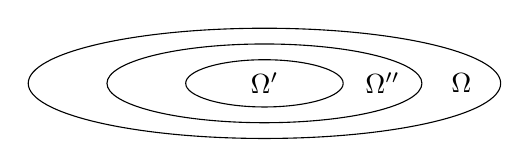
\begin{tikzpicture}
            \draw (0,0) circle(1 and 0.3);
            \draw (0,0) circle(2 and 0.5);
            \draw (0,0) circle(3 and 0.7);

            \node at(0,0) {\(\Omega^{\prime} \)};
            \node at(1.5,0) {\(\Omega ^{\prime\prime} \) };
            \node at(2.5,0) {\(\Omega\) };

            
        \end{tikzpicture}
    \end{center}

    Let \(\zeta\) be a smooth cutoff function:

    \(\zeta \equiv 1\) in \(\Omega ^{\prime} \) 

    \(\zeta \equiv 0\) on \(\Omega \setminus \Omega ^{\prime\prime} \)
    
    \(0 \leq \zeta \leq 1\) 

    We have:

    \[
        \int_{\Omega} a_{ij}(x) u_{x_i} v_{x_j} + b_i(x) u_{x_i} v + c(x) uv \,\mathrm{d}x = \int_{\Omega} fv \,\mathrm{d}x 
    \]

    \(\forall v\in H^1_0(\Omega)\) 

    Note that,

    \[
        \int_{\Omega} a_{ij}(x) u_{x_i} v_{x_j} + \boxed{b_i u_{x_i}} v + \boxed{c u} v \,\mathrm{d}x = \int_{\Omega} fv \,\mathrm{d}x 
    \]

    Choose \(v = - D_k^{-h} (\zeta^2 D_k^h u)\) 

    in \(\Omega ^{\prime} \) where \(\zeta \equiv 1\) we have:

    \[
        v = - \left( D_k^{-h} \left( \frac{u(x+he_k)-u(x)}{h} \right)  \right) 
    \]

    \[
        = - \left( \frac{u(x-h e_k + h e_k) - u(x - he_k) - u(x + h e_k) + u(x)}{-h^2} \right) 
    \]

    \[
        = - \left( \frac{u(x+he_k)+ u(x-he_k) - 2u(x)}{h^2} \right) 
    \]
    
    Using this \(v\), we get:

    \[
        I = \int_{\Omega} - a_{ij} u_{x_i} D_k^{-h} (\zeta^2 D_k^h u)_{x_i} - b_i u_{x_i} D_k^{-h} (\zeta^2) - cu D_k^{-h} (\zeta^2 D_k^h u) \,\mathrm{d}x 
    \]

    \[
        = - \int_{\Omega} f D_k^{-h} (\zeta^2 D_k^h u) \,\mathrm{d}x 
    \]

    \[
        I = \int_{\Omega} D_k^h (a_{ij}u_{x_i}) \left( \zeta^2 D_k^h u_{x_i} + 2 \zeta \varphi_{x_j} D_k^h u \right)  \,\mathrm{d}x 
    \]

    \[
        = \int_{\Omega} \left( a_{ij}(x+he_k) D_k^h(u_{x_i}) + D_k^h (a_{ij})u_{x_i} \right) \left( \zeta^2 D_k^h u_{x_j} + 2 \zeta \varphi_{x_j}D_k^h u \right)  \,\mathrm{d}x 
    \]

    \[
        = \int_{\Omega} \zeta^2 a_{ij}(x+he_k) D_k^h (u_{x_i}) D_k^h (u_{x_j}) + \text{others } \,\mathrm{d}x 
    \]

    \[
        \geq \theta \int_{\Omega} \zeta^2 \vert D_k^h (\nabla u) \vert ^ 2 + \text{ others }  \,\mathrm{d}x 
    \]

    Write \(\tilde{f} \coloneqq f - b_i u_{x_i} - cu \in L^2\).

    Weak form becomes:

    \[
        \int_{\Omega} a_{ij}(x) u_{x_i} v_{x_j} \,\mathrm{d}x = \int_{\Omega} \tilde{f}v \,\mathrm{d}x 
    \]

    We have:

    \[
        \theta \int_{\Omega} \zeta ^2 \vert D_k^h (\nabla u) \vert ^2 \,\mathrm{d}x \leq \int_{\Omega} \tilde{f} D_k^{-h} (\zeta^2 D_k^h u) - a_{ij}(x+he_k) 2 \zeta \zeta _{x_j} D_k^h(u_{x_i})D_k^h u  
    \]
    
    \[
        - D_k^h (a_{ij})u_{x_i}\zeta^2 D_k^h u_{x_j} - D_k^h (a_{ij}) u_{x_i} 2 \zeta \zeta_{x_j} D_k^h u \,\mathrm{d}x 
    \]

    Use \(ab \leq \varepsilon^2 a^2 + \frac{1}{4 \varepsilon^2} b^2\) to estimate terms 2,3,4.

    \[
        \leq C \int_{\Omega^{\prime\prime} } \left( \vert D_k^h (\nabla u) \vert \vert D_k^h u \vert + \vert D^h_k (\nabla u) \vert \vert \nabla u \vert + \vert \nabla u \vert \vert D_k^h u \vert \right) \zeta \,\mathrm{d}x 
    \]

    Note: \(C \to \infty \) as \(\Omega ^{\prime\prime} \to \Omega\) since it involves the derivative of the cutoff function.

\section*{Monday, 10/14/2024}

Recall: weak formulation:

\[
    \int_{\Omega} a_{ij} u_{x_i} v_{x_i} \,\mathrm{d}x = \int_{\Omega} fv - b_i u_{x_i} - cuv \,\mathrm{d}x 
\]

\[
    \eqqcolon \int_{\Omega} \tilde{f} v \,\mathrm{d}x, \tilde{f}\in L^2(\Omega)
\]

Choose: \(v = - D^{-h} _k (\zeta^2 D_k^h u)\) 

Start with LHS.

We arrived at:

\[
    LHS = \int_{\Omega} a_{ij} (x+he_k)D^h_k D^h _{k} (u_{x_{j}}) \zeta^2 \,\mathrm{d}x
\]

\[
    + \int_{\Omega} \bigg[ a_{ij}(x+he_k) 2 \zeta \zeta_{x_i} D_k^h u D_k^h (u_{x_i})+ D_k^h (a_{ij}) 2 \zeta \zeta _{x_j} D_k^h (u) u_{x_i} 
\]

\[    
    + D_k^h (a_{ij}) u_{x_i} D_k^h (u_{x_j}) \zeta^2 \bigg]  \,\mathrm{d}x  
\]

\[
    \implies LHS \geq \theta \int_{\Omega} \vert D^h(\nabla u) \vert ^2 \zeta^2 \,\mathrm{d}x 
\]

\[
    - C \left\{ \int_{\Omega} \vert D_k^ u \vert \vert D_k^h (\nabla u) \vert + \vert D_k^h u  \vert \vert \nabla u \vert + \vert D_k^h (\nabla u) \vert \vert \nabla u \vert \, \mathrm{d}x  \right\} 
\]

Now use \(\left( \varepsilon a - \frac{1}{2 \varepsilon} b \right) ^2 \geq 0 \implies ab \leq \varepsilon^2 a^2 + \frac{1}{4 \varepsilon^2} b^2 \) 

Now use our lemmas.

\[
    LHS \geq \theta \int \vert D^h (\nabla u) \vert ^2 - \varepsilon^2 \vert D_k^h (\nabla u) \vert ^ 2 - C_{\varepsilon} \vert \nabla u \vert ^ 2
\]

Pick \(\varepsilon^2 = \frac{\theta}{2}\) 

\[
    LHS \geq \frac{\theta}{2} \int_{\Omega} \vert D^h_k (\nabla u) \vert^2 \zeta^2\,\mathrm{d}x - C_{\varepsilon} \int_{\Omega} \vert \nabla u \vert ^ 2 \,\mathrm{d}x 
\]

Now we estimate RHS with a little of \(L^2\) norm \(v\) + a lot of \(L^2\) norm \(\tilde{f}\) 

By lemma 1:

\[
    \int v^2 \leq \int \vert \nabla (\zeta^2 D_k^h u) \vert ^ 2
\]

\[
    \leq  C \int \vert D_k^h \vert ^ 2 + \vert D_k^h (\nabla u) \vert ^ 2 \, \mathrm{d}x
\]

\[
    v \tilde{f}\, \mathrm{d}x\leq \varepsilon^2 \int v^2 + C_{\varepsilon} \int \tilde{f} ^2
\]

Pick \(\varepsilon^2 = \frac{\theta}{4}\) 

\[
    \implies \frac{\theta}{4} \int_{\Omega ^{\prime} } \left\vert D_k^ (\nabla u) \right\vert ^ 2 \,\mathrm{d}x \leq C \int_{\Omega} (f^2 + \vert \nabla u\vert^2 + u^2) \,\mathrm{d}x 
\]

\[
    \leq C \int_{\Omega} f^2 + \lVert u \rVert ^2 _ {H^1(\Omega)} \,\mathrm{d}x 
\]


Apply Lemma 2

\(u\in H^2_{loc} (\Omega)\) and \(\forall \Omega ^{\prime} \subset \subset \Omega\) 

\[
    \int_{\Omega^{\prime}} \vert D^2 u \vert ^ 2 \,\mathrm{d}x \leq  C \left( \lVert f \rVert ^ 2 _{L^2(\Omega)} + \lVert u \rVert ^ 2 _{H^1(\Omega)} \right) 
\]

Finally, we need to replace \(\lVert u \rVert ^2 _{H^1}\) with \(\lVert u \rVert ^2_{L^2}\) on RHS.

Using a new cut-off function \(\zeta\) such that \(\zeta \equiv 0\) on \(\Omega \setminus \Omega^{\prime\prime}\), we have:

\[
    \lVert u \rVert _{H^2(\Omega^{\prime})} \leq C \left( \lVert f \rVert ^ 2_{L^2(\Omega^{\prime\prime})} + \lVert u \rVert ^2 _{H^1(\Omega ^{\prime\prime} )} \right) 
\]

Now go back to \((\ast)\) weak formulation:

Choose \(v = \zeta ^2 u\)

\[
    \int_{\Omega} a_{ij} u_{x_i} u_{x_j} \zeta ^ 2 + a_{ij} u_{x_i} 2 \zeta \zeta_{x_i}  \,\mathrm{d}x = \int \tilde{f} \zeta^2 u
\]

Again, by ellipticity and \(ab \leq \varepsilon a ^ 2 + C_{\varepsilon} b^2\),

Choosing \(\varepsilon\) small in terms of \(\theta\),

\[
    \int_{\Omega^{\prime}} \vert \nabla u \vert ^ 2 \,\mathrm{d}x \leq C \int_{\Omega^{\prime\prime} } f^2 + u^2 \,\mathrm{d}x 
\]

so we're done!

\end{proof}

\section*{Wednesday, 10/16/2024}

\subsection*{Higher Interior Regularity}

Suppose \(Lu \coloneqq -(a_{ij} u_{x_i})_{x_j} + b_i(x) u_{x_i} + c(x) u\) 

So far: Assume \(a_{ij} \) elliptic, \(a_{ij} \in C^1\), \(b_i, c \in C^{\infty}\) \(f\in L^2(\Omega)\).

Then if \(u\in H^1(\Omega)\) is a weak solution to \(L u = f\) then \(u\in H^2_{\operatorname{loc}} (\Omega)\) and \(\forall \Omega ^{\prime} \subset \subset \Omega \exists C(\Omega ^{\prime} )\) such that:

\[
    \lVert u \rVert _{H^2(\Omega^{\prime})} \leq C(\Omega ^{\prime} ) ( \lVert f \rVert _{L^2} + \lVert u \rVert _{L^2})
\]

What if \(a_{ij}, b_i, c\) are \underline{nicer}, as is \(f\)? Then \(u\) should be \underline{nicer}.

Idea: Consider the PDE satisfied (weakly) by \(u_{x_k}\) for some \(k\in \{ 1, \cdots , n \}\).

\[
    \frac{\partial}{\partial x_k} L(u) = \frac{\partial}{\partial x_k} f
\]

\[
    - (a_{ij}(x) (u_{x_k})_{x_i})_{x_j} - (a_{ij} (x))_{x_k} (u_{x_k})_{x_i} + (b_i(x))_{x_k} u_{x_i} + b_i(x)(u_{x_k})_{x_i} 
\]
\[
    + (c(x))_{x_k} u + c(x) u_{x_k} = f_{x_k} 
\]

This is not exactly allowed. So we express it weakly.

Then \(u_{x_k} \) weakly solves a \underline{new} elliptic PDE.

\begin{theorem}
    Let \(m\) = non-neg integer. Assume \(a_{ij} , b_i, c \in C^{m+1} (\Omega)\). Assume \(f\in H^m(\Omega)\) 
    
    Ten if \(u\in H^1(\Omega)\) is a weak solution to \(Lu = f\) we have:

    \[
        u \in H^{m+2}_{\operatorname{loc}} (\Omega)
    \]

    and \(\forall \Omega ^{\prime} \subset \subset \Omega\) 
    
    \[
        \lVert u \rVert _{H^{m+2}(\Omega^{\prime})} \leq C (\lVert f \rVert _{H^m} + \lVert u \rVert _{L^2})
    \]
\end{theorem}

\begin{proof}
    By induction.
\end{proof}

\subsection*{Boundary Regularity}

\begin{theorem}
    Take \(\Omega \subset \mathbb{R}^n\), open, bounded, \(\partial \Omega \in C^2\). Take \(a_{ij}\) elliptic, \(a_{ij} \in C^1, b_i, c \in L^{\infty}\).

    Take \(f\in L^2\).

    Then if \(u\in H^1_0(\Omega)\) is a weak solution to \(Lu = f\) in \(\Omega\) and \(u=0\) on \(\partial \Omega\) then,

    \[
        u\in H^2(\Omega)
    \]

    \[
        \lVert u \rVert _{H^2(\Omega)} \leq C (\lVert f \rVert _{L^2} + \lVert u \rVert _{L^2})
    \]
\end{theorem}

\begin{proof}

    First we assume the boundary is flat. If not we flatten the boundary

    Suppose first that \(B(0,1) \cap \Omega = B(0,1) \cap \mathbb{R}^n_+ = \{ x\in \mathbb{R}^n \mid x_n > 0 \}\). 

    % insert picture figure

    Let \(\zeta\) be a cutoff function.

    \(\zeta \in C^{\infty}, \zeta \equiv 1\) in \(B(0,\frac{1}{2})\)

    \(\zeta \equiv 0\) in \(\mathbb{R}^n \setminus B(0,1)\)

    \[
        B[u,v] = \int fv \, \forall v \in H^1_0(\Omega)
    \]

    Rewrite:

    \[
        \int_{\Omega} a_{ij} u_{x_i} v_{x_j} \,\mathrm{d}x = \int_{\Omega} \widetilde{f} v \,\mathrm{d}x 
    \]

    For \(\vert h \vert \) small take:

    \[
        v = - D_k^{-h} (\zeta^2 D_k^h u)
    \]

    for any \(k\in \{ 1, \cdots , n-1 \} \) 

    To be a legal \(v\) for this, we need \(v\in H^1_0(\Omega)\) in light of the cut-off function and \(\eval{\Tr}_{\partial B(0,1)^+} u = 0 \) 

    So we can use this \(v\) in \(\ast\).

    The rest of the proof is the same for interior regularity. We obtain:

    \[
        \lVert D_k^h (\nabla u) \rVert _{L^2(B(0,1)^+)} \leq C \left( \lVert f \rVert _{L^2} + \lVert u \rVert _{L^2} \right) 
    \]

    Since difference quotients are uniformly bounded we must have weak derivatives.

    \(\implies\) by lemma 2,

    \[
        \lVert u_{x_i x_j} \rVert \leq C \left( \lVert f \rVert _{L^2} + \lVert u \rVert _{L^2} \right)
    \]

    for all \(i,j\) except \(i=j=n\).

    How to control \(u_{x_n x_n}\)?

    By interior regularity, \(L u = f\) at a.e. \(x\in \Omega\).

    We rewrite the PDE:

    \[
        - a_{n n} u_{x_n x_n} = \underbrace{\sum_{(i,j) \neq (n,n)} (a_{ij} (x) u_{x_i})_{x_j}  - b_i(x) u_{x_i} - c(x)u + f}_{\coloneqq \tilde{\tilde{f}}}
    \]

    We have \(\lVert \tilde{\tilde{f}} \rVert < \operatorname{const}(\lVert f \rVert _{L^2} + \lVert u \rVert _{L^2})\) 

    \[
        \implies \lVert u_{x_n x_n}  \rVert \leq \frac{\operatorname{const}}{\theta} \left( \lVert f \rVert _{L^2} + \lVert u \rVert _{L^2} \right) 
    \]

    \section*{Friday, 10/18/2024}
    

    We have proved the theorem for flat portion of \(\partial \Omega\). For proving the general case, we flatten the boundary.

    Locally write \(\partial \Omega\) as a graph:

    \[
        x_n = f(x_1, \cdots , x_{n-1}) \, f \in C^2
    \]

    We change variables.

    \[
        y_j = x_j \, j = 1, \cdots , n-1
    \]

    \[
        y_n = x_n - f(x_1, \cdots , x_{n-1})
    \]

    \[
        y = \Phi(x)
    \]

    [insert picture figure]

    Then,

    \[
        D \Phi (x) = \begin{bmatrix}
            1 & 0 & \cdots &  0 \\
            0 & 1 & \cdots &  0 \\
            \vdots & \vdots & \ddots  &  \vdots \\
            - f_{x_1} & -f_{x_2} & \cdots & 1
        \end{bmatrix}
    \]

    \(\det D \Phi = J \Phi = 1\).

    By inverse function theorem, \(\Phi\) is invertible. Let \(\Psi = \Phi ^{-1}\). Define:

    \[
        \widetilde{u} (y) \coloneqq u(\Psi(y))
    \]

    \[
        u(x) = \widetilde{u}(\Phi(x))
    \]

    By chain rule,

    \[
        u_{x_i} = \widetilde{u}_{y_k} \Phi_{x_i} ^{(k)}
    \]

    Weak form:

    \[
        \int_{\Phi(B(x_0,R)\cap \Omega)} \left(\underbrace{a_{ij} (\Psi(y))\widetilde{u}_{u_k} \Phi_{x_k} ^{(k)} \widetilde{v}_{y_l} \Phi_{x_j}^{(l)}}_{\widetilde{a}_{kl} \widetilde{u}_{y_k} \widetilde{v}_{y_l} } + b_i (\Psi(y))\widetilde{u}_{x_k} \Phi^{(k)}_{x_i} + c(\Psi(y)) \widetilde{u}  \right) \cdot 1  \,\mathrm{d}y 
    \]

    \[
        = \int_{\Phi(B(x_0,R)\cap \Omega)} f(\psi(y))\widetilde{v}(y) \,\mathrm{d}y 
    \]

    \underline{Claim}: \(\widetilde{u}\) solves an elliptic PDE weakly on a \underline{flat} domain.

    Define \(\widetilde{a}_{kl}(y) \coloneqq a_{ij} \Phi^{(k)}_{x_i} \Phi^{(l)}_{x_j}\).
    
    We're done one we check that:

    \[
        \widetilde{a}_{kl} = \widetilde{a}_{lk}, \widetilde{a_{kl}} \eta _k \eta_l \geq \widetilde{\theta} \vert \eta \vert ^ 2 \, \forall \eta \in\mathbb{R}^n
    \]

    Firstly,

    \[
        \widetilde{a}_{lk} = a_{ij} \Phi^{(l)}_{x_i} \Phi^{(k)}_{x_j} = a_{ji} \Phi^{(l)}_{x_i}\Phi^{(k)}_{x_j} = \widetilde{a}_{kl}
    \]

    Then let \(\eta\in\mathbb{R}^n\).

    \[
        \widetilde{a}_{kl} \eta_k \eta_l = a_{ij} \Phi^{(k)}_{x_i} \Phi^{(l)}_{x_j} \eta_k \eta_l = a_{ij} \underbrace{\Phi_{x_i}^{(k)}\eta_k}_{=\xi_i} \underbrace{\Phi^{(l)}_{x_j}\eta_l}_{=\xi_j} \geq \theta \vert \xi \vert ^ 2
    \]

    Let \(\xi_i = \Phi^{(k)}_{x_i} \eta_k\) and \(\xi_j = \Phi^{(l)}_{x_j} \eta_l\).
    
    Then, \(\xi = D \Phi \eta \implies (D \Phi)^{-1} \xi = \eta \implies D \Psi \xi = \eta\).
    
    \[
        \vert \eta \vert \leq \vert D \Psi \vert \vert \xi \vert \leq C_{d \Omega} \vert \xi \vert 
    \]

    Therefore,

    \[
        \widetilde{a}_{kl} \eta_k \eta_l \geq \theta \vert \xi \vert ^ 2 \geq \frac{\theta}{C_{\partial \Omega}} \vert \eta \vert ^ 2
    \]

    So, this reduces to the case of flat boundary, which we have already proven.

\end{proof}

\subsection*{Maximum Principles}

Consider \(L\) in non-divergence form:

\[
    Lu \coloneqq -a_{ij}(x) u_{x_i x_j} + b_i(x) u_{x_i} + c(x)u 
\]

\begin{theorem}
    [Weak Maximum Principle] Assume \(u\) is a `nice classical solution', meaning \(u\in C^2(\Omega)\cap C(\overline{\Omega})\) for some bounded open \(\Omega \subset \mathbb{R}^n\).
    
    Further assume \(c(x)\equiv 0\) in the definition of \(L\).

    \begin{enumerate}[label=\roman*)]
        \item If \(Lu \leq 0\) in \(\Omega\) then,
        \[
            \max_{\overline{\Omega}} u = \max_{\partial \Omega} u
        \]
        \item If \(Lu \geq 0\) in \(\Omega\) then,
        \[
            \min_{\overline{\Omega}} u = \min_{\partial \Omega} u
        \]
    \end{enumerate} 
\end{theorem}

\underline{Remarks}:

\begin{enumerate}[label=\arabic*)]
    \item  If \(L u \leq 0\) we call \(u\) a subsolution. If \(Lu \geq 0\) we call \(u\) a supersolution.

    \item If \(Lu = 0\) then both maximum and minimum are achieved on the boundary.

    \item A weak maximum principle does not preclude the max also being achieved inside \(\Omega\).
    
    \item If \(c\not\equiv 0\), the maximum principle may \underline{fail}.
    
    \underline{Example}: If \(\Omega = (0,\pi)\) and \(Lu = -u^{\prime\prime} - u = 0\) then \(a_{11} = 1, b_1 = 0, c(x)=-1\). For Dirichlet boundary condition \(u(0)=u(\pi)=0\). Our answer can be \(\sin x\). Then the maximum happens at \(\frac{\pi}{2}\) not in boundary for \(A > 0\). 

\end{enumerate}

\section*{Monday, 10/21/2024}

\underline{Recap}:

\[
    Lu \coloneqq -a_{ij} (x) u_{x_i x_j} + b_{i} () u_{x_i} + c(x) u_{i}  
\]

\(a_{ij}\) uniformly elliptic \(a_{ij} (x) \xi_i \xi_j \geq \theta \vert \xi \vert ^ 2, \theta > 0, a_{ij} = a_{ji}. a_{ij}, b_i, c\) are continuous on \(\overline{\Omega}, \Omega \subset \mathbb{R}^n\) is open bounded.

Then we have the weak maximum principle as shown above. 

\begin{proof}
    Case 1: Suppose \(Lu < 0\) [strictly less than \(0\)]. We proceed by contradiction to show a \underline{strong maximum principle}.

    Suppose \(\exists x_0 \in \Omega\) such that \(u(x_0)=\max_{\overline{\Omega}} u(x)\).

    Consider \(Lu(x_0)\). Note that \(\eval{u_{x_i}}_{x_0} = 0\) since \(\nabla u(x_0)=0\). Thus,

    \[
        Lu(x_0) = -a_{ij}(x_0) u_{x_i x_j}(x_0)  
    \]

    \underline{Linear Algebra Fact}: If a matrix \(A\) is symmetric positive definite then \(A\) can be diagonalizable by an orthogonal matrix \(\mathcal{O}\) so that \(\mathcal{O} \mathcal{O}^T = I\). Then,
    
    \[
        \mathcal{O} A \mathcal{O}^T = \begin{bmatrix}
            \lambda_1 & \cdots &  0 \\
            \vdots & \ddots & \vdots  \\
            0 & \cdots &  \lambda_n \\
        \end{bmatrix}
    \]

    \[
        \lambda_1, \cdots , \lambda_n > 0
    \]

    Assume \(u\in C^2\) and has a min at \(x_0\).

    Change variables: \(y = x_0 + \mathcal{O} (x - x_0)\). Then,

    \[
        u_{x_i} = u_{y_k} \mathcal{O}_{ki}
    \]

    \[
        u_{x_i x_j} = u_{y_k y_l} \mathcal{O}_{ki} \mathcal{O}_{lj}
    \]

    \[
        a_{ij} (x_0) u_{x_i x_j}(x_0) = \sum_{i,j} \left[ \sum_{k,l} a_{ij} (x_0) u_{y_k y_l} \mathcal{O}_{ki} \mathcal{O}_{lj}  \right] 
    \]

    \[
        = \sum_{k,l} u_{y_k y_l} \left[ \sum_{i,j} a_{ij} (x_0) \mathcal{O}_{ki} \mathcal{O}_{lj} \right]
    \]

    \[
        = \sum_{k,l} u_{y_k y_l} (\mathcal{O} A) \mathcal{O}_{jl}^T u_{y_k y_l} (x_0) = \lambda_1 u_{y_1 y_1} + \cdots + \lambda_n u_{y_n y_n} 
    \]

    At a max, \(u_{y_j y_j} \leq 0\) for all \(j\). Then \(Lu(x_0) \geq 0\) which gives us the contradiction.

    \underline{Case 2}: Suppose \(Lu \leq 0\). We pertrub \(L\) to get back to the first case. For example:

    \[
        u^{\epsilon} (x) \coloneqq u(x) + \epsilon e^{\lambda x_1}
    \]

    \[
        L u^{\epsilon} = \underbrace{Lu}_{\leq 0} + L(\epsilon e^{\lambda x_1}) \leq - \epsilon \lambda^2 a_{11} (x) e^{\lambda x_1}+\epsilon b_1(x)\lambda e^{\lambda x_1}
    \]

    \[
        = \epsilon \lambda e^{\lambda x_1} (-\lambda a_{11} (x) + b_1(x)) \leq \epsilon e^{\lambda x_1}(-\theta \lambda + \lVert b \rVert _{L^{\infty}})
    \]

    Pick \(\lambda\) big enough so that \(L u^{\epsilon} < 0\). By case 1,
    
    \[
        \max_{\overline{\Omega}} u \leq  \max_{\overline{\Omega}}u^{\epsilon} (x) = \max_{\partial \Omega} u^{\epsilon} (x) \leq \max_{\partial \Omega} u + \epsilon \max_{\partial \Omega} e^{\lambda x_1} \leq \max_{\partial \Omega} u + \epsilon e^{\lambda R}
    \]

    where \(\Omega \subset B(0,R)\). Let \(\epsilon \to 0\) to finish the proof.

\end{proof}

Now we try to make sense of the case \(c(x) \geq 0\).

\begin{theorem}
    [Weak max princ. for \(c(x)\geq 0\)]

    Assume \(u\in C^2(\Omega)\cap C(\overline{\Omega})\).

    Assume \(c(x) \geq 0 \forall x\in \Omega\).

    \begin{enumerate}[label=\roman*)]
        \item If \(Lu \leq 0\) in \(\Omega\) then \(\max_{\overline{\Omega}} u \leq \max_{\partial \Omega} u^+\)
        \item If \(Lu \geq 0\) in \(\Omega\) then \(\min_{\overline{\Omega}}u \geq - \max_{\partial \Omega}u^-\)   
    \end{enumerate} 

    Where \(u^+(x) \coloneqq \max (u(x),0), u^-(x) = -\min (u(x),0)\).
\end{theorem}

\underline{Note}: If \(Lu = 0\) had a solution, then \(\max_{\overline{\Omega}} \vert u \vert = \max_{\partial \Omega} \vert u \vert \) 

\underline{Example}: Let \(Lu = - u^{\prime\prime} + (4x^2 + 1)u\).

\(b_i \equiv 0, c(x) = 4x^2 + 1 > 0\) 

\(\Omega = (-1,1)\).

Consider \(u(x) = e^{-x^2} - 4\)

\(u^{\prime} = -2x e^{-x^2}\)

\(u^{\prime\prime} = -2 e^{-x^2} + 4x^2 e^{-x^2}\) 

\(L u =(2-4x^2)e^{-x^2} + (4x^2 + 1)(e^{-x^2} - 4) = 3 e^{-x^2} - 16x^2 - 4 < 0 \) on \((-1,1)\) 

Max of \(u\) comes in the origin, which is \(-3\). But it is not at the boundary! We need to be careful about the sign and positive part and negative parts.

\begin{proof}
    Let \(\Omega ^{\prime} = \{ x\in \Omega : u(x) > 0 \}\).

    \(\Omega ^{\prime} = \varnothing \implies u(x) \leq 0\) in \(\overline{\Omega}\) so we're done.

    If \(\Omega ^{\prime} \neq \varnothing\) then we have:

    [picture figure]

    Let \(Ku \coloneqq L u - c(x)u\), and \(K\) doesn't have the \(c\) term. So we can apply theorem 1 to \(\Omega ^{\prime} \). 

    \[
        Ku \leq - c(x) u \leq 0 \, \text{in } \Omega ^{\prime} 
    \]

    \[
        \max_{\overline{\Omega}} u \leq \max_{\overline{\Omega^{\prime}}} u \leq \max_{\partial \Omega ^{\prime}} u = \max_{\partial \Omega} u^+ 
    \]

    In \(\partial \Omega\) for the negative part \(u^+ \equiv 0\) so we can ignore that boundary, we're done!

\end{proof}

\section*{Wednesday, 10/23/2024}

\begin{lemma}
    [Hopf Lemma]

    Assume \(u\in C^2(\Omega)\cap C^1(\Omega)\) and assume \(c(x) \equiv 0\) Suppose \(L u \leq 0\) in \(\Omega\) and \(\exists x_0\in \partial \Omega\) such that:

    \(u(x_0) > u(x) \forall x\in \Omega\)and

    \(\Omega\) satisfies an interior ball condition at \(x_0\), namely \(\exists y_0 \in \Omega, \exists r > 0\) such that \(B(y_0, r) \subset \Omega\) with \(x_0 \in \partial B(y_0, r)\).

    Then \(\frac{\partial u}{\partial \nu} (x_0) > 0\) where \(\nu = \frac{x_0 - y_0}{\vert x_0 - y_0 \vert }\) [outer normal].

    If \(c(x) \geq 0\) then the same conclusion holds provided \(u(x_0) \geq 0\).

    [pictures / fig bad example]

    A \underline{sufficient} condition for this to hold: if the boundary is given by a \(C^2\) function [so the curvature never gets too extreme] it is enough for the boundary to be \(C_2\).

\end{lemma}

\underline{Note}: \(\frac{\partial u}{\partial \nu} (x_0) \geq 0\) is immediate since \(u(x_0) > u(x) \forall x\in \Omega\).

So the significance is the \underline{strict inequality}.

\begin{proof}
    Define \(v(x) = e^{-\lambda \vert x \vert ^2} - e^{-\lambda r^2}\), \(\lambda > 0\) to be specified later.

    \[
        v_{x_i} = - 2 \lambda x_i e^{-\lambda \vert x \vert ^ 2} 
    \]

    \[
        v_{x_i x_j} = (4 \lambda^2 x_i x_j - 2 \lambda \delta_{ij})e^{-\lambda \vert x \vert^2}
    \]

    \[
        Lv = - a_{ij}(x) ( 4\lambda ^2 x_i x_j - 2 \lambda \delta_{ij}) e^{-\lambda \vert x \vert ^ 2} - 2 \lambda b_i (x) x_i e^{-\lambda \vert x \vert^2} + c(x) e^{-\lambda \vert x \vert^2} - c(x) e^{-\lambda r^2}  
    \]

    \[
        \implies Lv \leq \left( - 4 \lambda^2 \theta \vert x \vert ^ 2 + 2 \lambda \Tr A + 2 \lambda \vert b \vert _{L^{\infty}} \vert x \vert + \vert c \vert _{L^{\infty}}\right) e^{-\lambda \vert x^2 \vert} - \cancel{c(x) e^{-\lambda r^2}}
    \]

    This is \(< 0\) for some choice of \(\lambda  = \lambda(\theta , \Omega, \Tr A, \vert b \vert_{L^{\infty}}, \vert c \vert_{L^{\infty}})\) 

    WLOG \(y_0 = 0\). Consider the annulus:

    \[
        \left\{ x : \frac{r}{2} < \vert x \vert < r \right\} = \mathcal{A}
    \]

    [insert picture figure]

    \(\exists \varepsilon > 0\) such that:

    \[
        u(x_0) \geq u(x) + \varepsilon v(x) \, \forall x\in \partial B\left(0, \frac{r}{2}\right)
    \]

    since \(u(x_0) > \max_{\partial B(0, \frac{r}{2})} u\) 

    On \(\partial B(0,r)\):

    \[
        u(x_0) \geq u(x) + \varepsilon v(x) = u(x)
    \]

    Note \(L(u+\varepsilon v - u(x_0))\):

    \[
        = \underset{\leq 0}{Lu} + \underset{< 0}{\varepsilon L v} - \underset{\leq 0}{c(x) u(x_0)}  < 0
    \]

    And we've shown that \(u(x) + \varepsilon v(x) - u(x_0) \leq 0\) on \(\partial \mathcal{A}\).

    By weak maximum principle, 

    \[
        u(x) + \varepsilon v(x) - u(x_0) \leq 0 \, \text{in } \mathcal{A}
    \]

    Also note:

    \[
        u(x_0) + \varepsilon v(x_0) - u(x_0) = 0
    \]

    Therefore,

    \[
        \frac{\partial}{\partial \nu} (u(x) + \varepsilon v(x) - u(x_0)) \geq 0
    \]

    \[
        \implies \frac{\partial}{\partial \nu} u(x_{0}) \geq - \varepsilon \frac{\partial}{\partial \nu } v(x_0)
    \]

    Note that \(v\) is a radial function so \((-\varepsilon)\frac{\partial}{\partial \nu} v(x_0) = 2 \varepsilon \lambda (x_0) e^{-\lambda r^2} > 0\). 

\end{proof}

\begin{theorem}
    [Strong Maximum Principle]

    Assume \(\Omega \subset \mathbb{R}^n\) is open, bounded and connected. Assume \(u\in C^2(\Omega) \cap C^1(\overline{\Omega})\). 

    Suppose \(c\equiv 0\). 

    \begin{enumerate}[label=\roman*)]
        \item If \(L u \leq 0\) in \(\Omega\) and if \(u\) attains its maximum over \(\overline{\Omega}\) at an interior point, then \(u\equiv \text{const}\).
        \item If \(L u \geq 0\) in \(\Omega\) and if \(u\) attains its minimum over \(\overline{\Omega} \) at an interior point then \(u\equiv \text{const}\). 
    \end{enumerate} 
\end{theorem}

\begin{proof}
    Let \(M \coloneqq \max_{\overline{\Omega}} u\). Let \(S \coloneqq \{ x\in \Omega : u(x) = M \}\).
    
    If \(S = \Omega\) we're done.

    If \(S = \varnothing\) then we're done.

    So suppose, by contradiction, \(S \neq \Omega , \varnothing\).

    [insert picture]

    Choose \(y \in \Omega \setminus S\) so that:

    \[
        \operatorname{dist}(y,S) < \operatorname{dist}(y, \partial \Omega)
    \]

    Draw the largest open ball \(B\)  centered at \(y\) that doesn't intersect \(S\).

    Necessarily, \(\exists x_0 \in \partial B \cap S\).

    Thus \(\Omega \setminus S\) satisfies an interior ball condition at \(x_0\).

    \(u(x_0) > u(x) \forall x\in \Omega \setminus S\).

    We apply Hopf lemma.

    The outer normal derivative \(\frac{\partial u}{\partial \nu} (x_0) > 0\).

    This cannot be true, since \(\frac{\partial u}{\partial \nu} (x_0) = \nabla u(x_0) \cdot \nu = 0\) since \(\nabla u(x_0) = 0\) at an internal max.
\end{proof}

\section*{Friday, 10/25/2024}

\begin{theorem}
    [Strong Maximum Principle with \(c(x) \geq 0\)]

    Assume \(\Omega \subset \mathbb{R} ^ n\), bounded open with \(\partial \Omega \subset C^2\). Assume \(u\in C^2(\Omega)\cap C^1(\overline{\Omega})\).

    \begin{enumerate}[label=\roman*)]
        \item If \(Lu \leq 0\) in \(\Omega, u\) achieves a non-negative max inside \(\Omega\) then \(u\equiv \text{const}\).
        \item If \(Lu \geq 0\) in \(\Omega, u\) achieves a non-positive min inside \(\Omega\) then \(u\equiv \text{const}\).
    \end{enumerate} 
\end{theorem}

\begin{proof}
    Identical to \(c\equiv 0\) case.
\end{proof}

\subsection*{Uniqueness}

For \(Lu = f, c(x) \geq 0, u=0\) on \(\partial \Omega\) we have seen a uniqueness result.

\begin{theorem}
    \(\Omega \subset \mathbb{R}^n\) open bounded an \(\partial \Omega \in C^2\).Suppose \(u_1\) and \(u_2\) both solve \(Lu = f\) in \(\Omega\) with \(c(x)\equiv 0\) and \(\nabla u \cdot \nu = g\) on \(\partial \Omega\) where \(\nu =\) outer unit normal.

    Then \(u_1 - u_2 \equiv \text{const}\).
\end{theorem}

\begin{proof}
    Let \(v \coloneqq u_1 - u_2\).

    Then \(Lv = Lu_1 - Lu_2 = f-f = 0\) in \(\Omega\).

    \[
        \nabla v \cdot \nu = \nabla u_1\cdot \nu - \nabla u_2\cdot \nu = g-g = 0 \, \text{on } \partial \Omega
    \]

    By the max principle either \(v\equiv \text{const}\) or \(v\) attains its max at a point \(x_0 \in \partial \Omega\).

    Then, \(v(x_0) > v(x) \forall x\in \Omega\).

    We can use Hopf Lemma:

    \[
        \nabla v(x_0) \cdot \nu > 0
    \]

    this is a contradiction, so we're done.
\end{proof}

\begin{theorem}
    Assume \(Lu \leq f\) in a open connected bounded domain \(\Omega \subset \mathbb{R}^n\) and assume \(c(x) \geq 0\).

    Assume \(u\in C^2(\Omega) \cap C(\overline{\Omega})\). Then,

    \[
        \max_{\overline{\Omega}} u \leq \max_{\partial \Omega} u^+ + C_1 \max_{\overline{\Omega}} f^+
    \]

    where \(C_1\) depends on the coefficients of \(L\) and \(\Omega\).

    If \(Lu = f\) then we can say

    \[
        \max_{\overline{\Omega}} \vert u \vert \leq \max_{\partial \Omega} \vert u \vert + C_1 \max_{\overline{\Omega}} \vert f \vert
    \]
\end{theorem}

\begin{proof}
    We use a Barrier construction.

    Without loss of generality let's assume

    \[
        \Omega \subset \{ x\in \mathbb{R}^n : 0 < x_1 < d \}
    \]

    for some \(d\).

    Let \(Ku \coloneqq Lu - cu = - a_{ij}(x) u_{x_i x_j} + b_i(x)u_{x_i}\).
    
    For \(\lambda > 0\) to be chosen let's compute

    \[
        K(e^{\lambda x_1}) = (- a_{11} (x) \lambda^2 + b_1 \lambda )e^{\lambda x_1} 
    \]

    \[
        \leq (-\theta \lambda^2 + \vert b \vert _{L^{\infty}}\lambda)e^{\lambda x_1}
    \]

    \[
        = - \theta \left( \lambda^2 - \frac{\lambda \vert b \vert _{L^{\infty}}}{\theta} \right) e^{\lambda x_1}
    \]

    \[
        \leq -\theta \, \text{for } \lambda \text{ large enough} 
    \]

    Goal: Pick a \(v\) such that \(L(u-v) \leq 0, u-v \leq 0\) on \(\partial \Omega\).

    Pick \(v(x) = \max_{\partial \Omega} u^+ + \left( \frac{e^{\lambda d} - e^{\lambda x_1}}{\theta} \right) \max_{\overline{\Omega}}f^+  \)
    
    \(Lv = Kv + cv \geq Kv\)
    
    \[
        = \frac{\max_{\overline{\Omega}}f^+}{\theta} K(e^{\lambda x_1}) \geq \max f^+
    \]

    Note: \(cv \geq 0\) since \(c \geq 0, v \geq 0\).

    Then, \(L(u-v) \leq f - \max f^+ \leq 0\).

    On \(\partial \Omega\),

    \[
        u - v = u - \max_{\partial \Omega} u^+ - \text{positive} \leq 0 
    \]

    By maximum principle,

    \[
        \max_{\overline{\Omega}} (u-v) \leq \max_{\partial \Omega} (u-v)^+ \leq 0
    \]

    Thus, \(u -v \leq 0 \implies u \leq v \leq \max_{\partial \Omega} u^+ + \frac{e^{\lambda d}}{\theta} \max_{\overline{\Omega}} f^+\).

    Choosing \(C_1 = \frac{e^{\lambda d}}{\theta}\) solves our problem.
\end{proof}

Recall that we had

\[
    \lVert u \rVert _{H^2(\Omega^{\prime})} \leq C \left( \lVert f \rVert _{L^2(\Omega)} + \lVert u \rVert _{L^2(\Omega)} \right) 
\]

\(\forall \Omega ^{\prime} \subset \subset ^{\prime} \Omega, C = C(\Omega ^{\prime} , \Omega)\).

If, for example \(L u = f\) in \(\Omega\) and \(u = h\) on \(\partial \Omega\) then,

\[
    \vert u \vert \leq \text{const}(f,h)
\]

\end{document}